\chapter{Analisi esplorativa del grafo}

\section{Obiettivi dell’analisi esplorativa}

Dopo la costruzione del grafo diretto pesato, è stata effettuata un’analisi esplorativa finalizzata a descriverne la struttura generale prima di passare a misure più avanzate di centralità e alle analisi strutturali. In particolare, questa fase si è concentrata su quattro aspetti principali:
\begin{itemize}
    \item le statistiche globali della rete;
    \item la distribuzione dei gradi dei nodi;
    \item l’individuazione degli aeroporti con più connessioni in ingresso e in uscita;
    \item lo studio delle componenti connesse della rete.
\end{itemize}

L’obiettivo è comprendere se la rete presenti una struttura distribuita in modo uniforme oppure se, come spesso avviene nelle reti di trasporto, emerga una configurazione di tipo \textit{hub-and-spoke}, caratterizzata da pochi nodi molto connessi e da molti nodi periferici con poche connessioni.

\section{Statistiche globali del grafo diretto}

L’analisi del grafo diretto conferma i risultati già emersi nella fase di costruzione. La rete risulta composta da 3425 nodi e 37595 archi, con una densità pari a circa 0.0032 e la presenza di un solo self-loop. La Tabella~\ref{tab:exploratory_summary} riassume le principali statistiche globali calcolate in questa fase.

\begin{table}[H]
\centering
\caption{Sintesi delle principali statistiche esplorative del grafo diretto.}
\label{tab:exploratory_summary}
\begin{tabular}{lc}
\toprule
\textbf{Statistica} & \textbf{Valore} \\
\midrule
Numero di nodi & 3425 \\
Numero di archi & 37595 \\
Densità & 0.0032058 \\
Numero di self-loops & 1 \\
Numero di weakly connected components & 8 \\
Numero di strongly connected components & 44 \\
Dimensione largest weakly connected component & 3397 \\
Dimensione largest strongly connected component & 3354 \\
Media in-degree & 10.9766 \\
Media out-degree & 10.9766 \\
Mediana in-degree & 3 \\
Mediana out-degree & 3 \\
Massimo in-degree & 238 \\
Massimo out-degree & 239 \\
\bottomrule
\end{tabular}
\end{table}

Il valore molto basso della densità mostra che la rete è fortemente sparsa: solo una piccola parte delle connessioni possibili tra aeroporti è effettivamente presente. Questo comportamento è del tutto plausibile nel contesto del trasporto aereo, poiché non tutti gli aeroporti sono direttamente collegati tra loro e il traffico tende a concentrarsi attorno a un numero limitato di hub principali.

\section{Visualizzazione globale della rete}

Per accompagnare i dati numerici con una rappresentazione visiva della struttura complessiva, sono state generate alcune visualizzazioni dell’intero grafo e delle sue componenti principali. Pur trattandosi di grafi molto densi, tali figure risultano utili per cogliere in modo immediato la presenza di una componente dominante, di una zona centrale fortemente concentrata e di nodi periferici disposti ai margini della rete.

\begin{figure}[H]
\centering
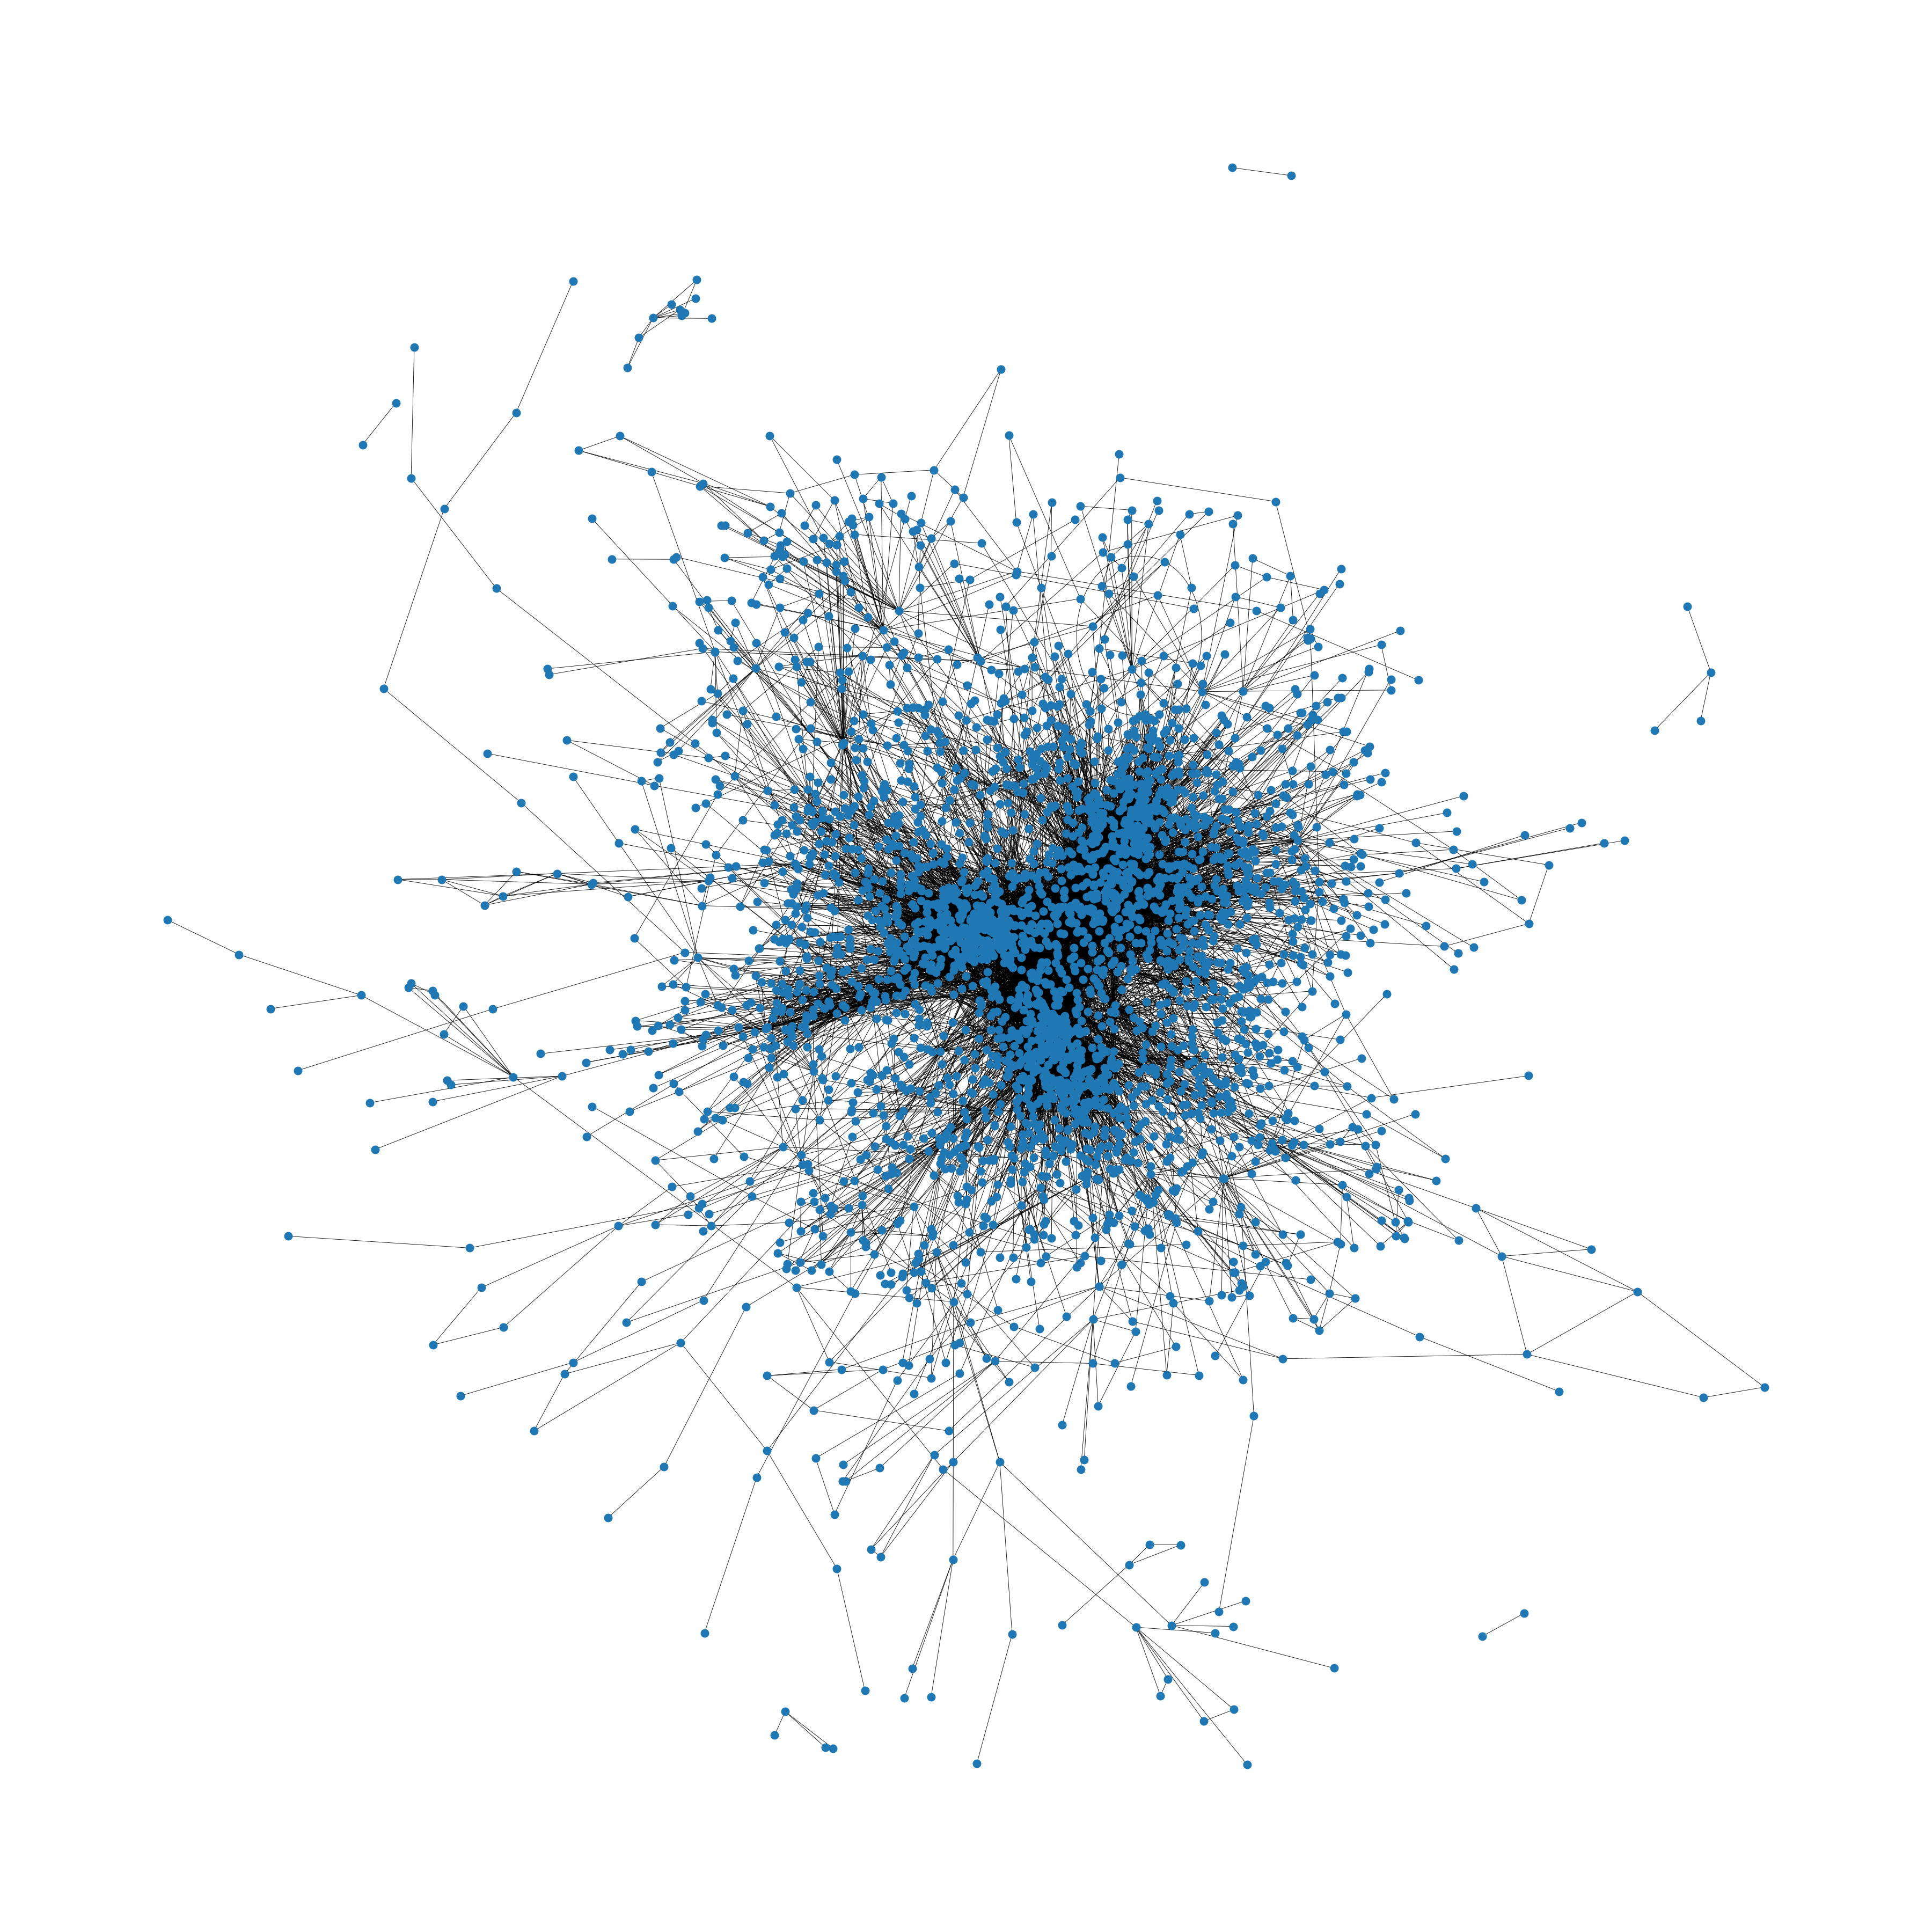
\includegraphics[width=0.9\textwidth]{chapter4/immagini/full_network_graph.png}
\caption{Visualizzazione globale della rete completa.}
\label{fig:full_network_graph}
\end{figure}

La Figura~\ref{fig:full_network_graph} mostra il grafo complessivo della rete. Anche se una rappresentazione di questo tipo non consente una lettura dettagliata dei singoli nodi, permette comunque di osservare chiaramente una forte concentrazione delle connessioni nella parte centrale del sistema e la presenza di diversi nodi o piccoli gruppi periferici disposti ai margini.

Per analizzare meglio la struttura principale della rete, sono state poi rappresentate separatamente la largest weakly connected component e la largest strongly connected component.

\begin{figure}[H]
\centering
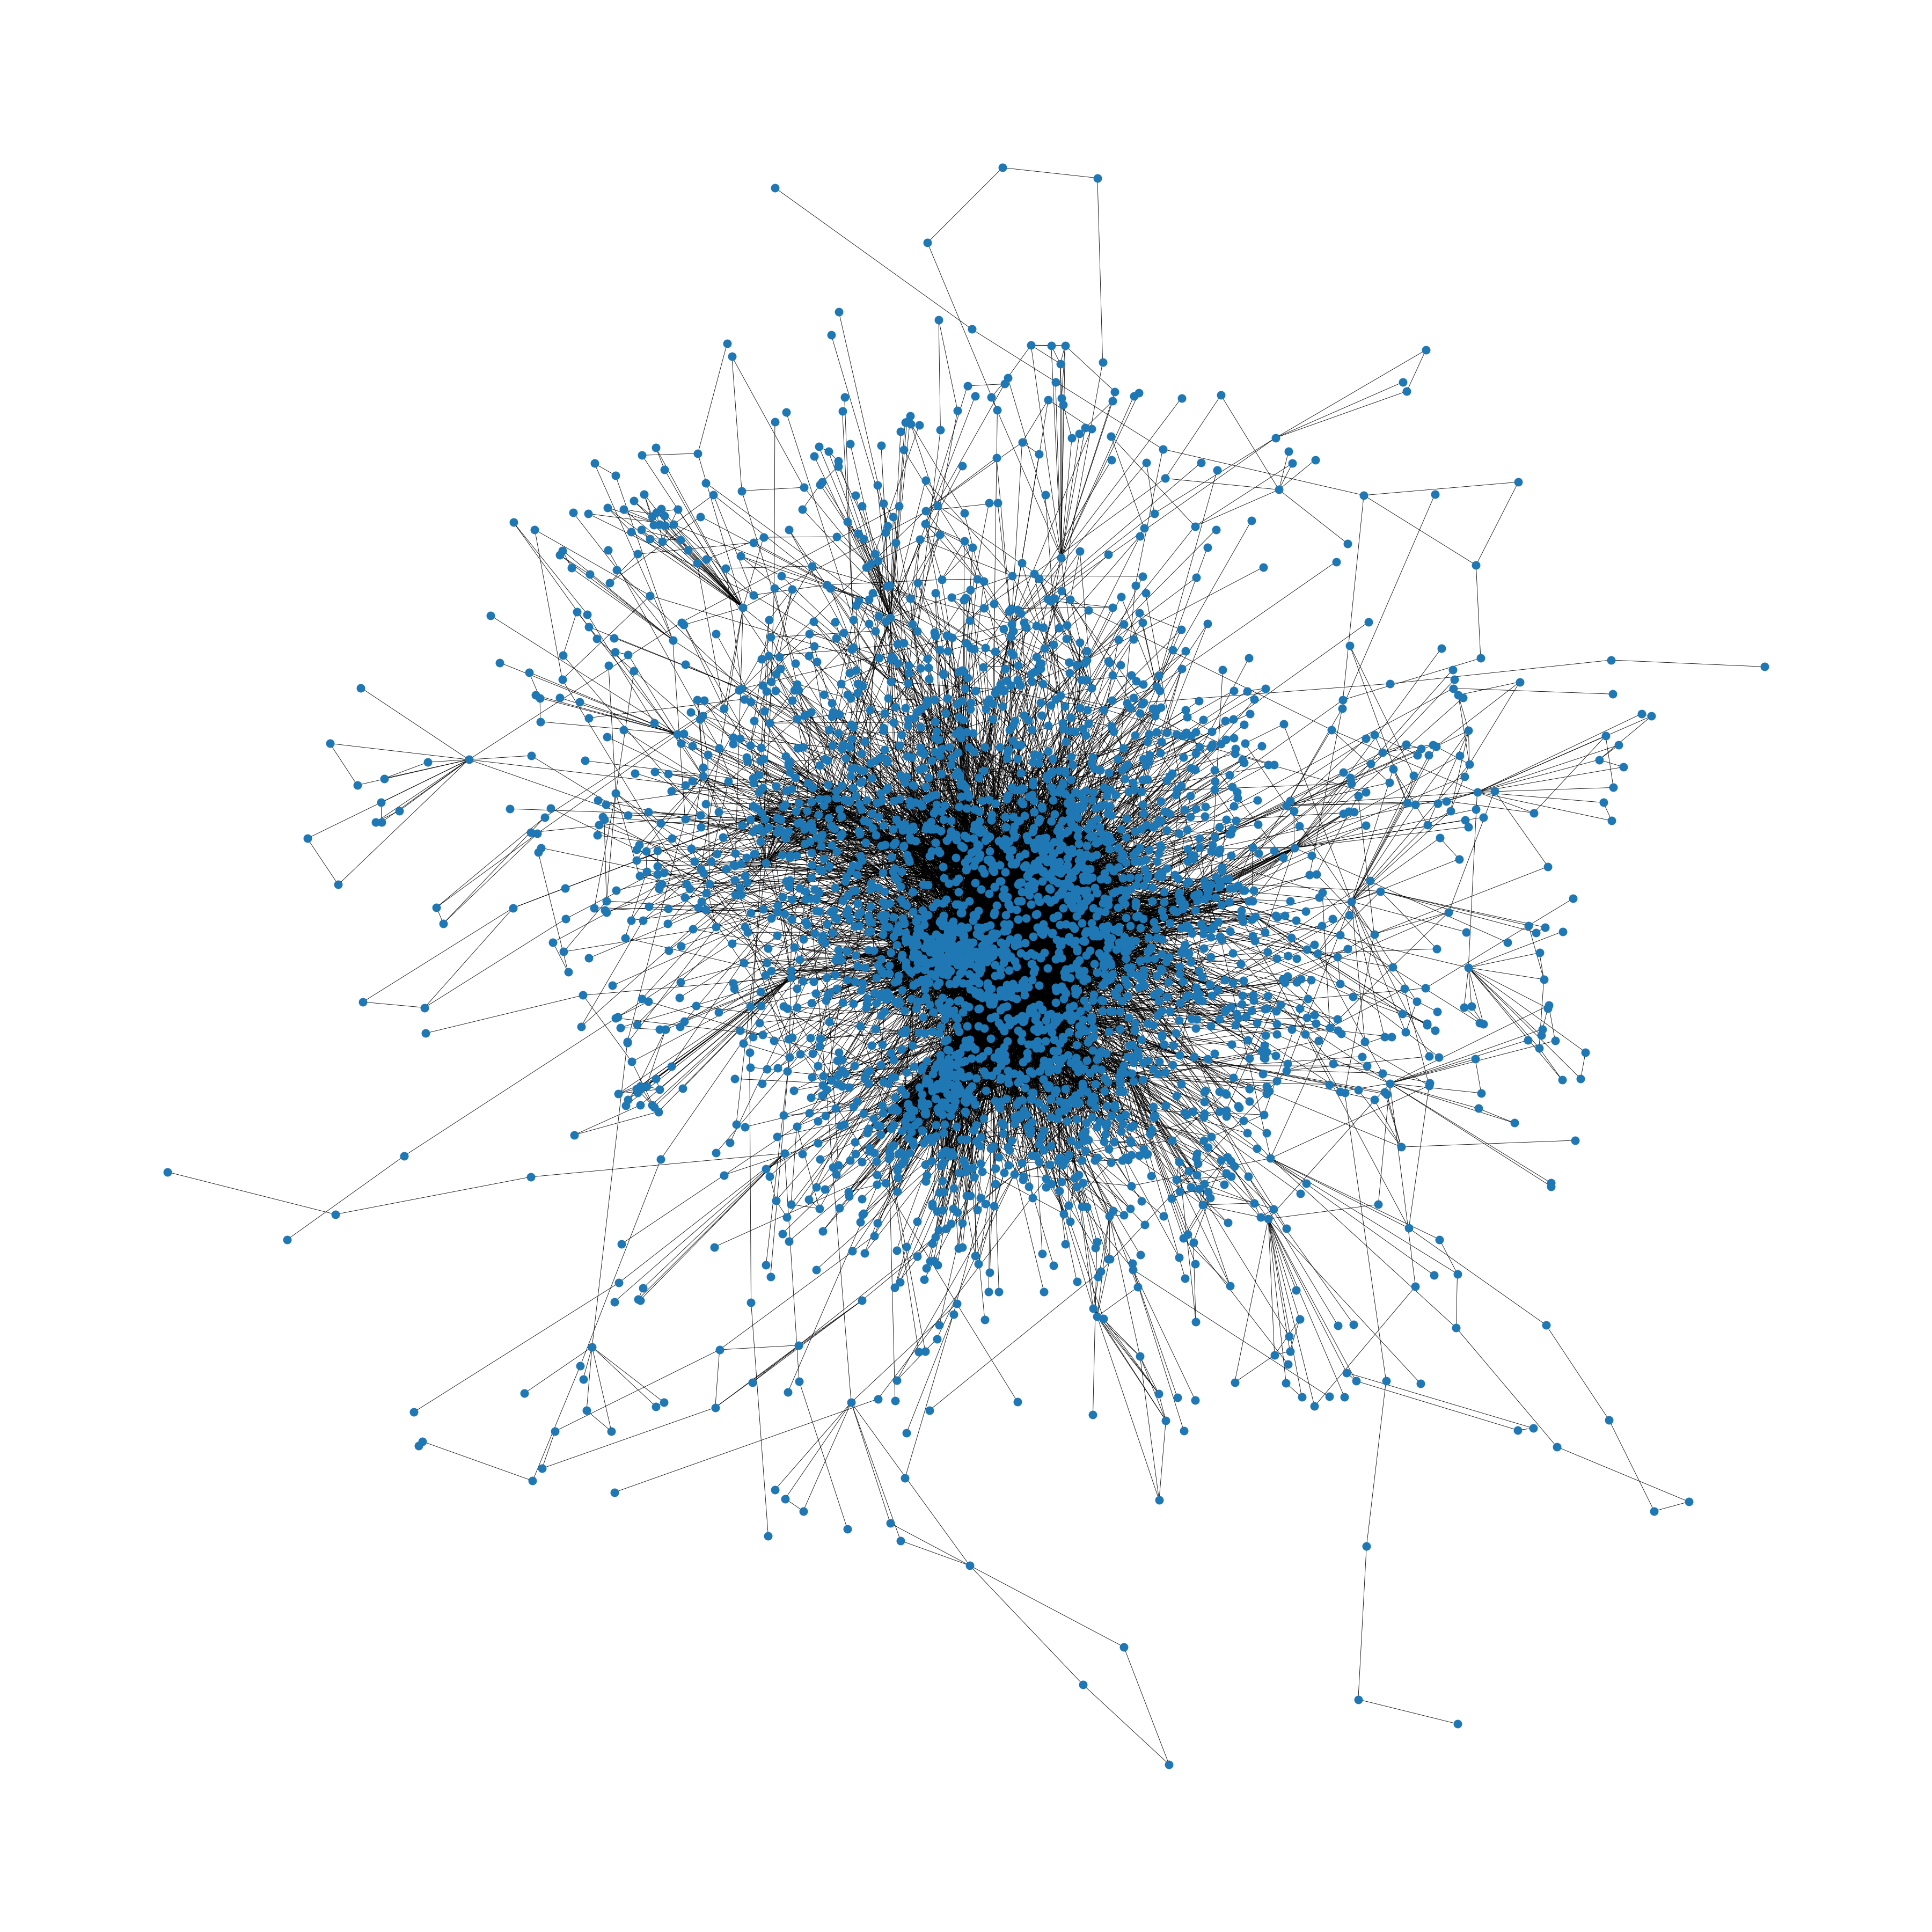
\includegraphics[width=0.9\textwidth]{chapter4/immagini/largest_weak_component_graph.png}
\caption{Visualizzazione della largest weakly connected component.}
\label{fig:largest_weak_component_graph}
\end{figure}

\begin{figure}[H]
\centering
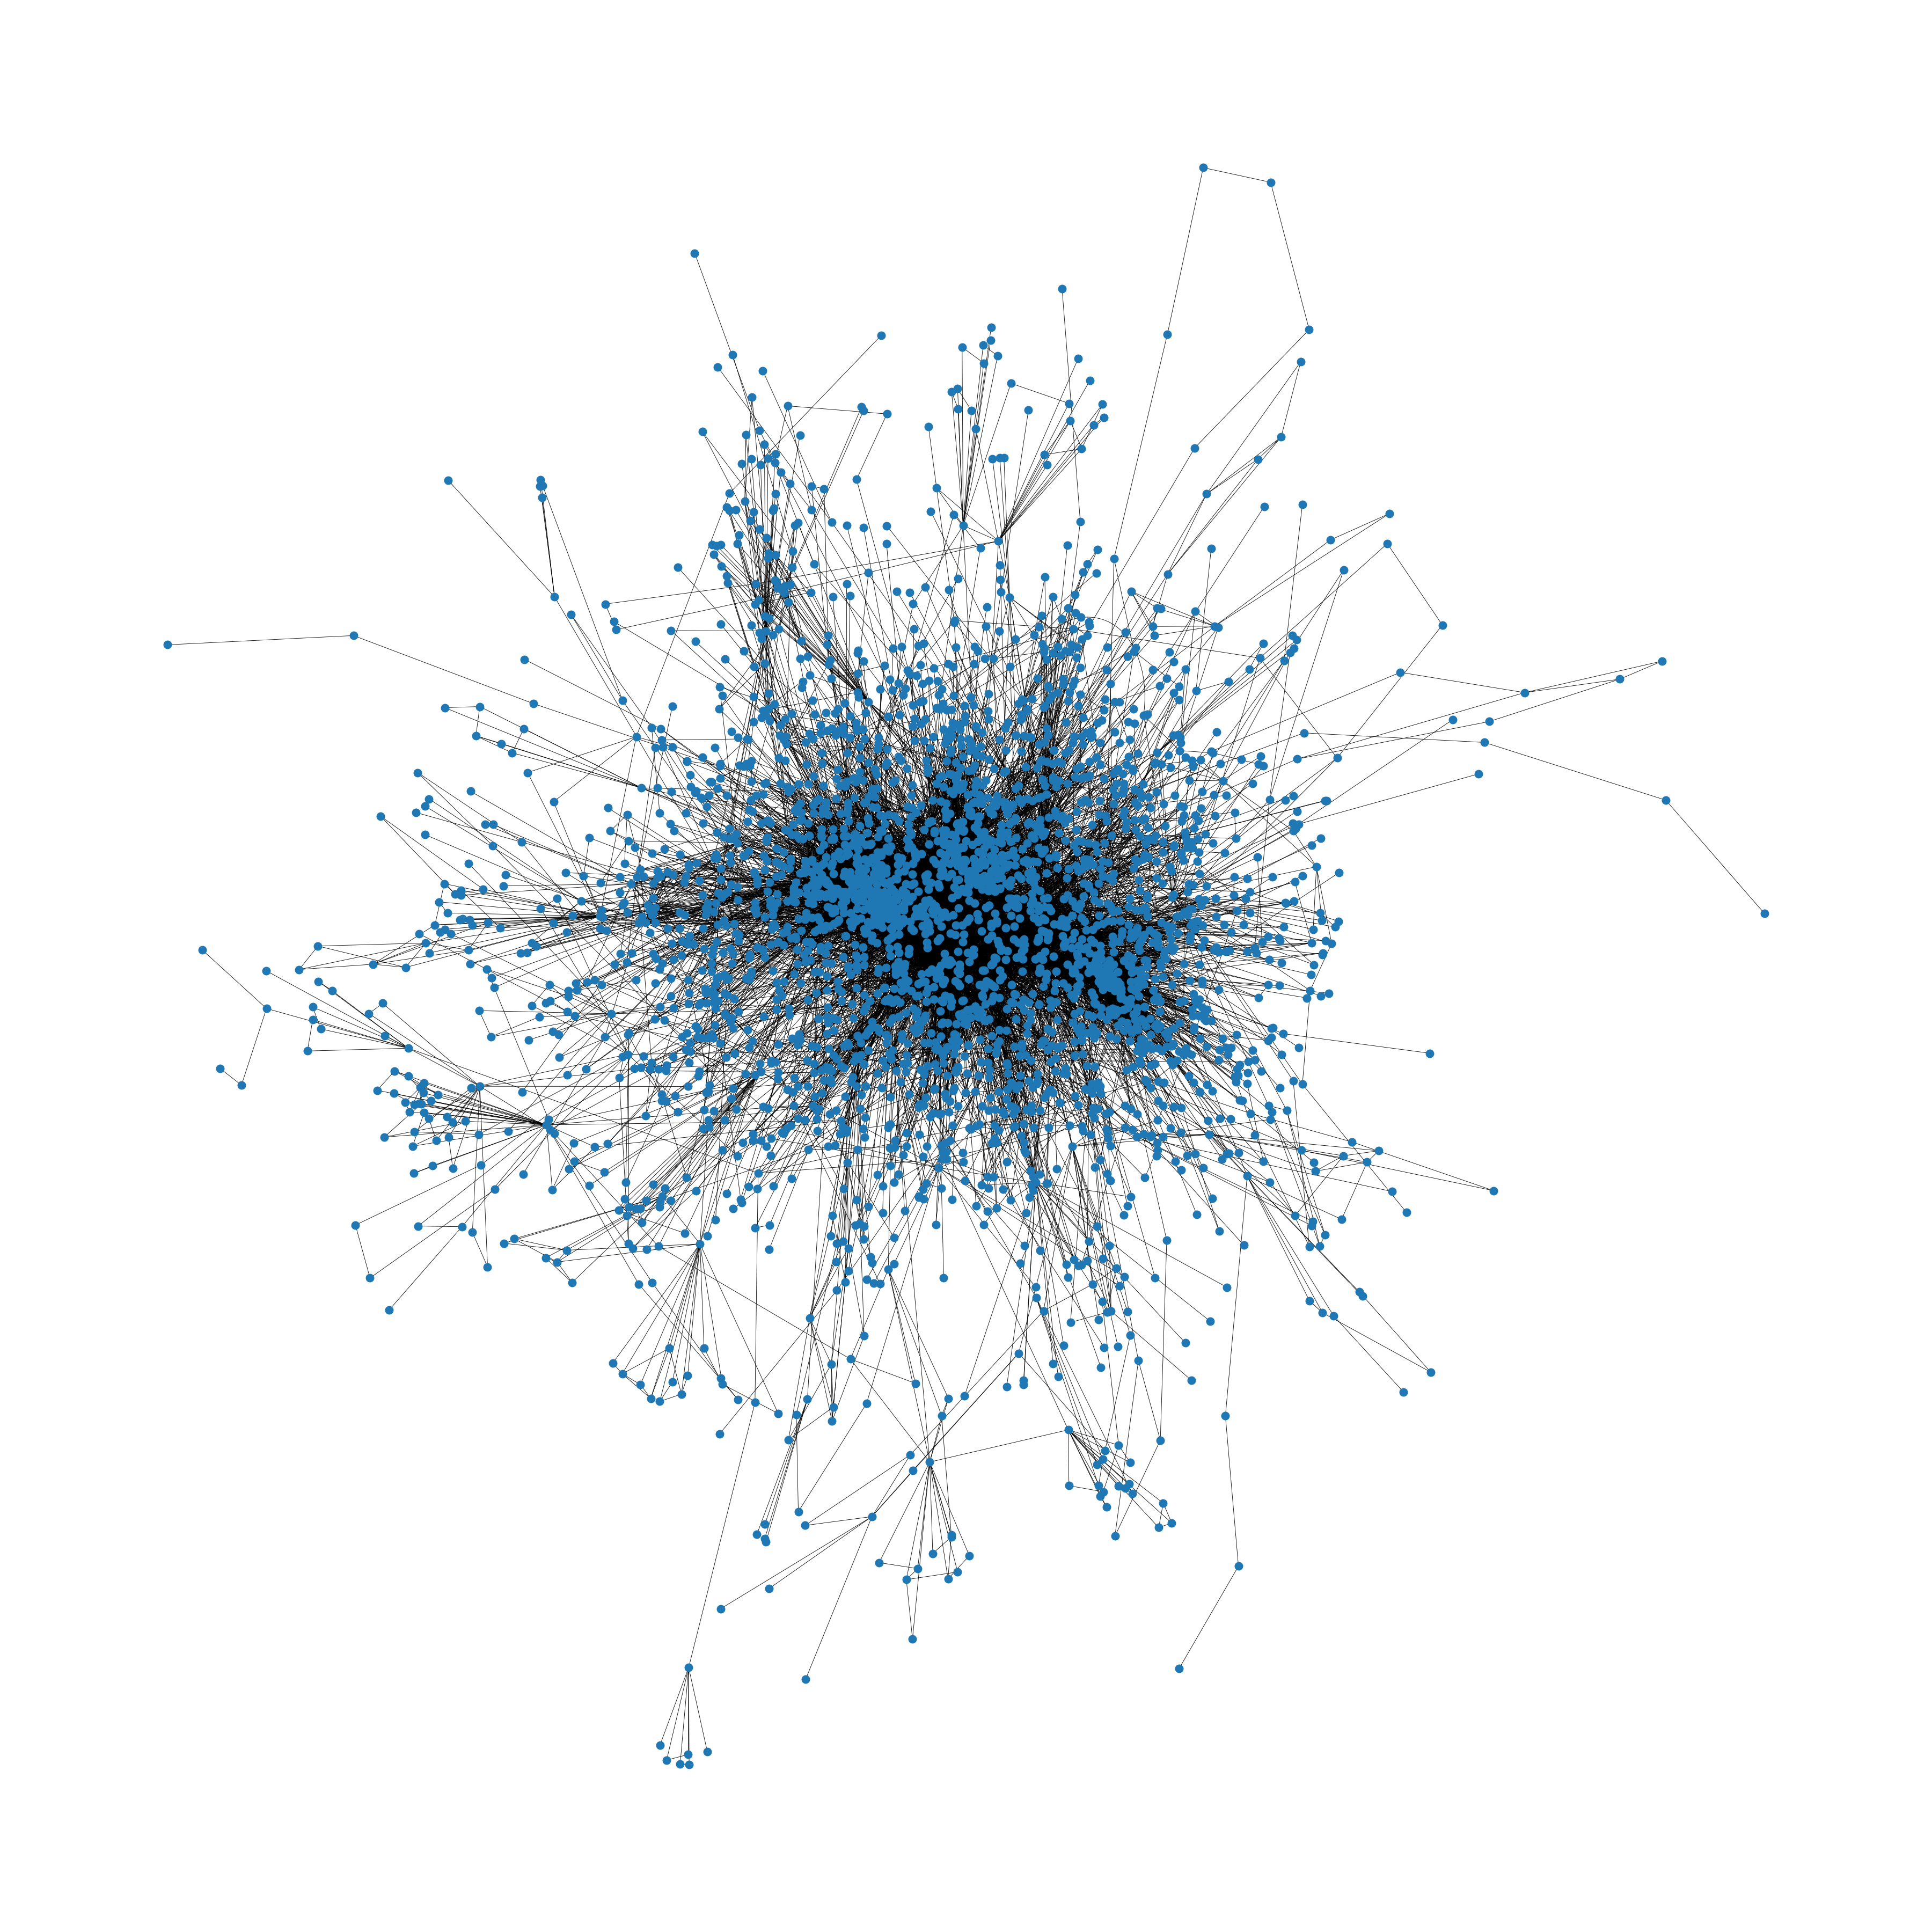
\includegraphics[width=0.9\textwidth]{chapter4/immagini/largest_strong_component_graph.png}
\caption{Visualizzazione della largest strongly connected component.}
\label{fig:largest_strong_component_graph}
\end{figure}

Le Figure~\ref{fig:largest_weak_component_graph} e~\ref{fig:largest_strong_component_graph} confermano visivamente quanto già osservato a livello quantitativo: la quasi totalità della rete appartiene a una componente principale molto estesa e fortemente integrata. La somiglianza tra le due strutture è coerente con il fatto che la largest strongly connected component possiede una dimensione molto vicina a quella della largest weakly connected component.

\section{Distribuzione dei gradi}

Per comprendere meglio la struttura della rete, sono state analizzate le distribuzioni di in-degree e out-degree. I grafici ottenuti mostrano una forte asimmetria: la maggior parte degli aeroporti presenta un numero ridotto di connessioni, mentre un numero ristretto di nodi raggiunge valori molto elevati.

\begin{figure}[H]
\centering
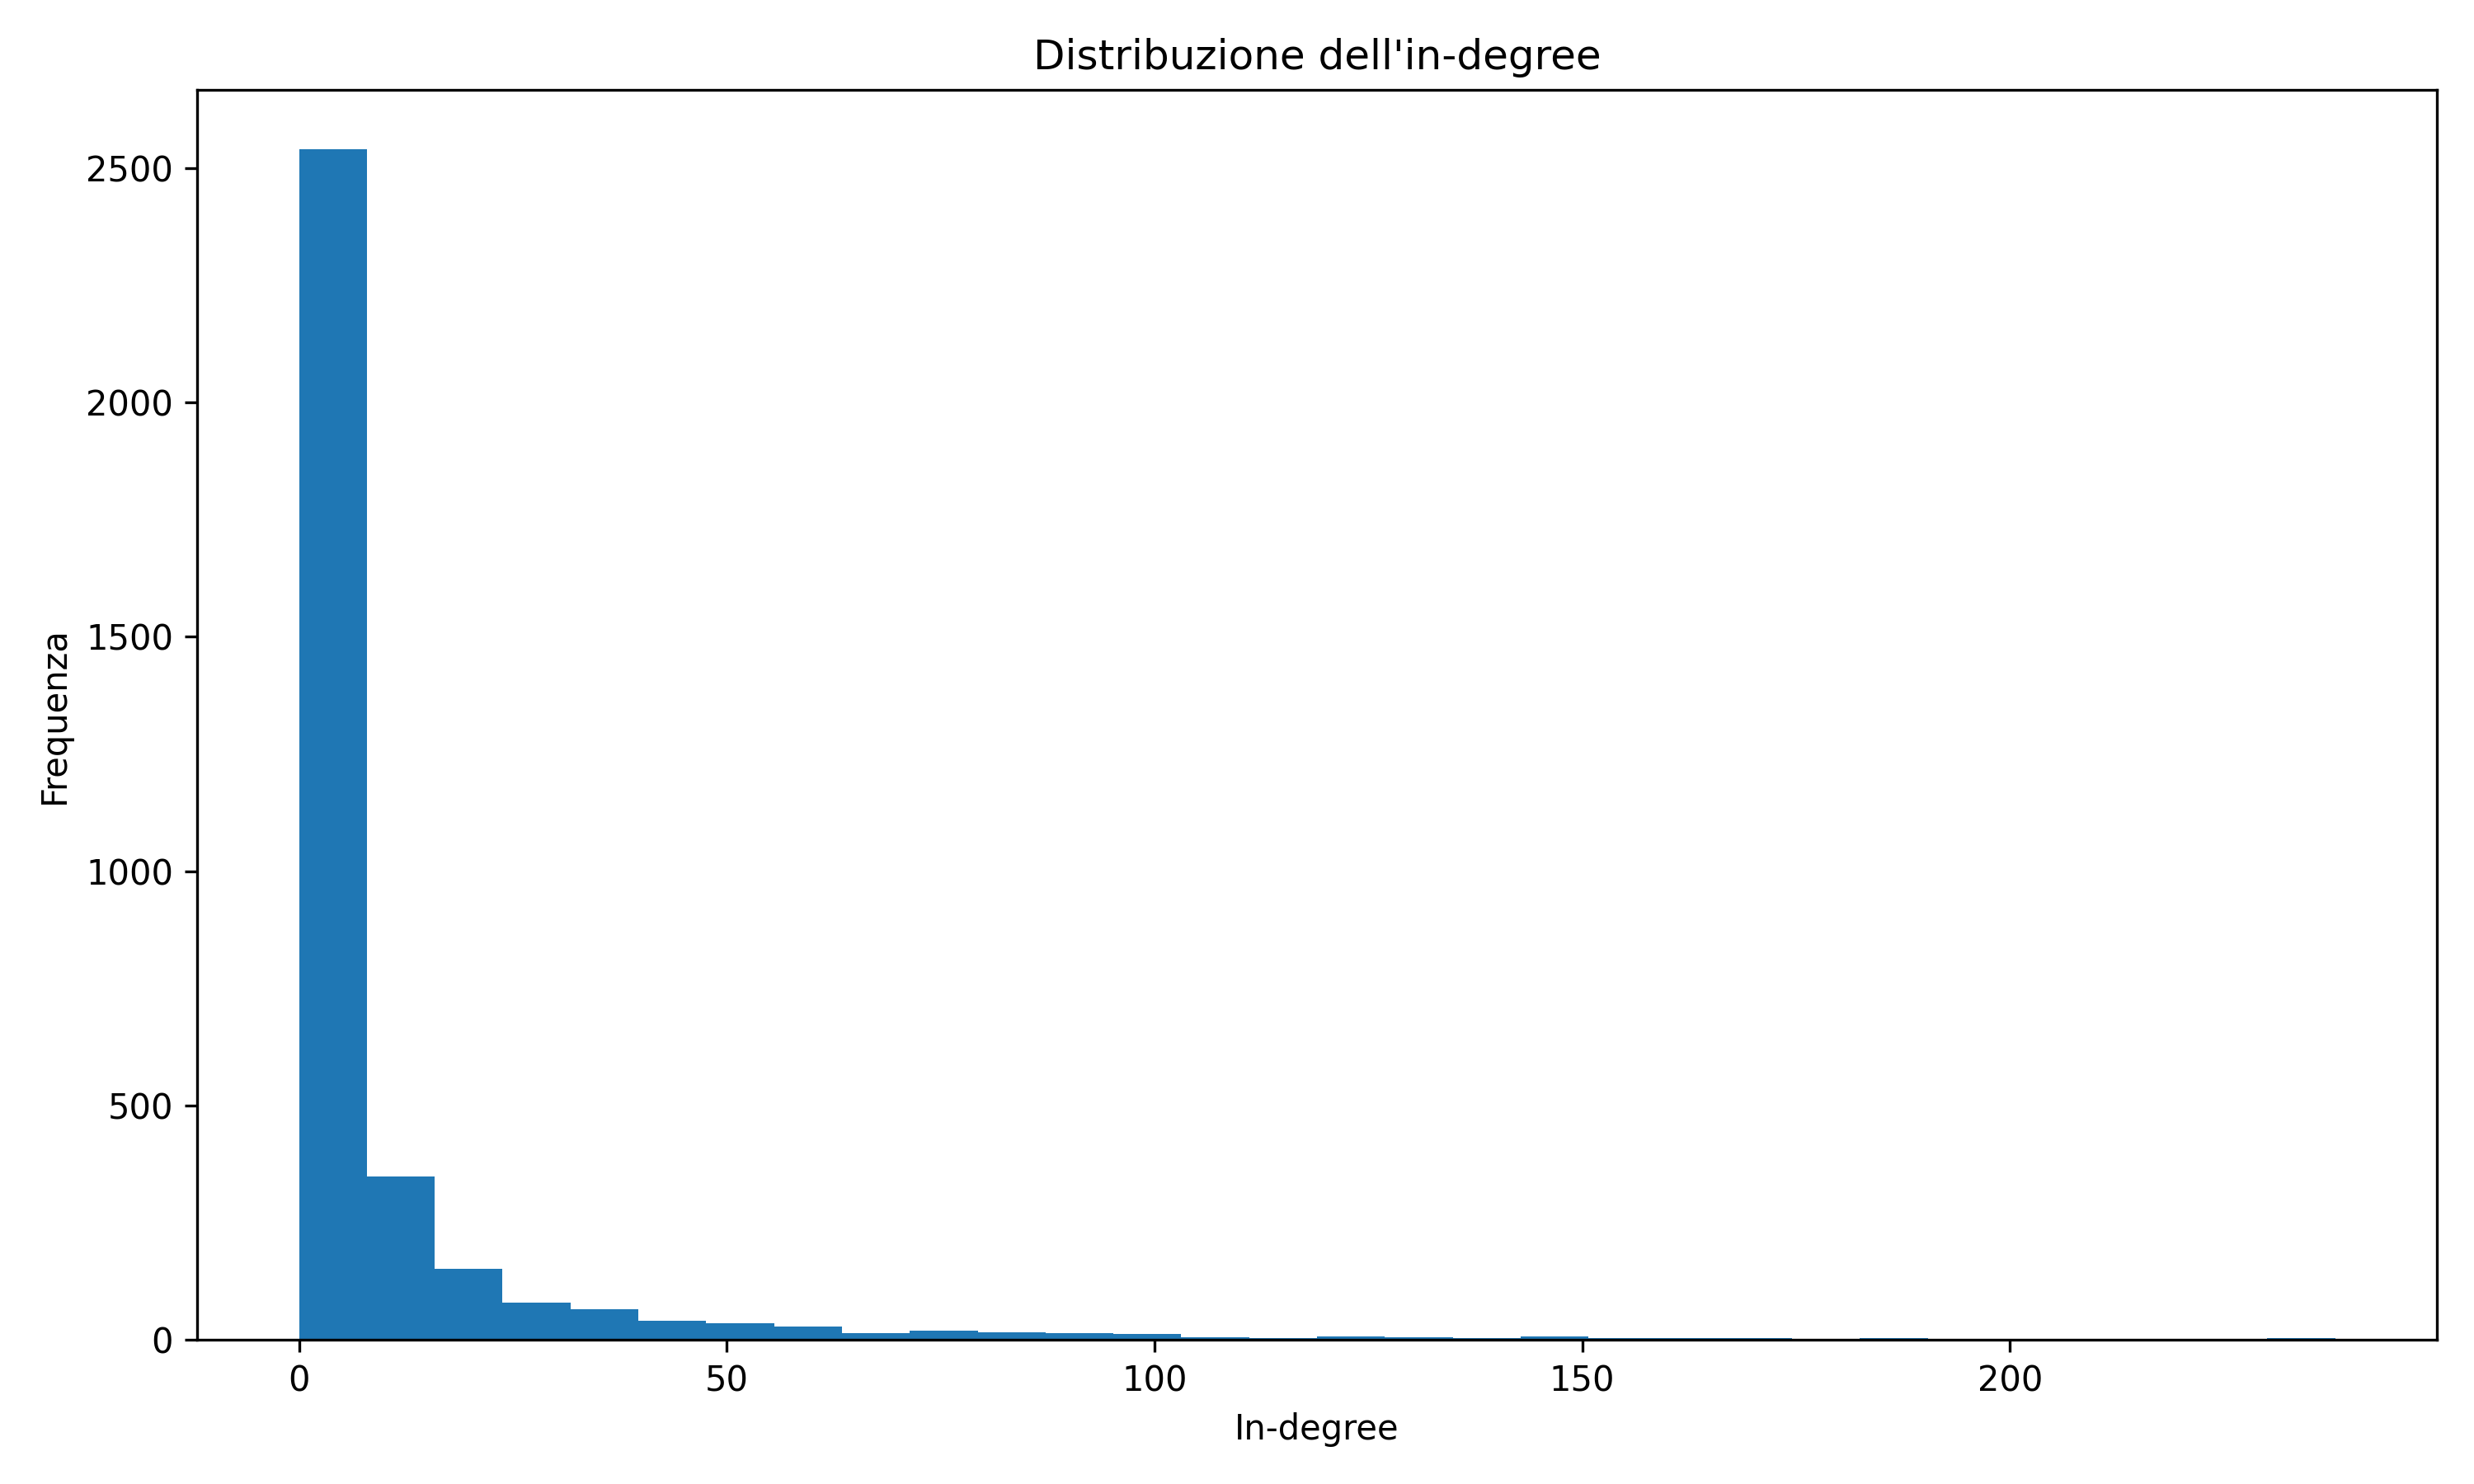
\includegraphics[width=0.9\textwidth]{chapter4/immagini/in_degree_distribution.png}
\caption{Distribuzione dell’in-degree nel grafo diretto.}
\label{fig:in_degree_distribution}
\end{figure}

\begin{figure}[H]
\centering
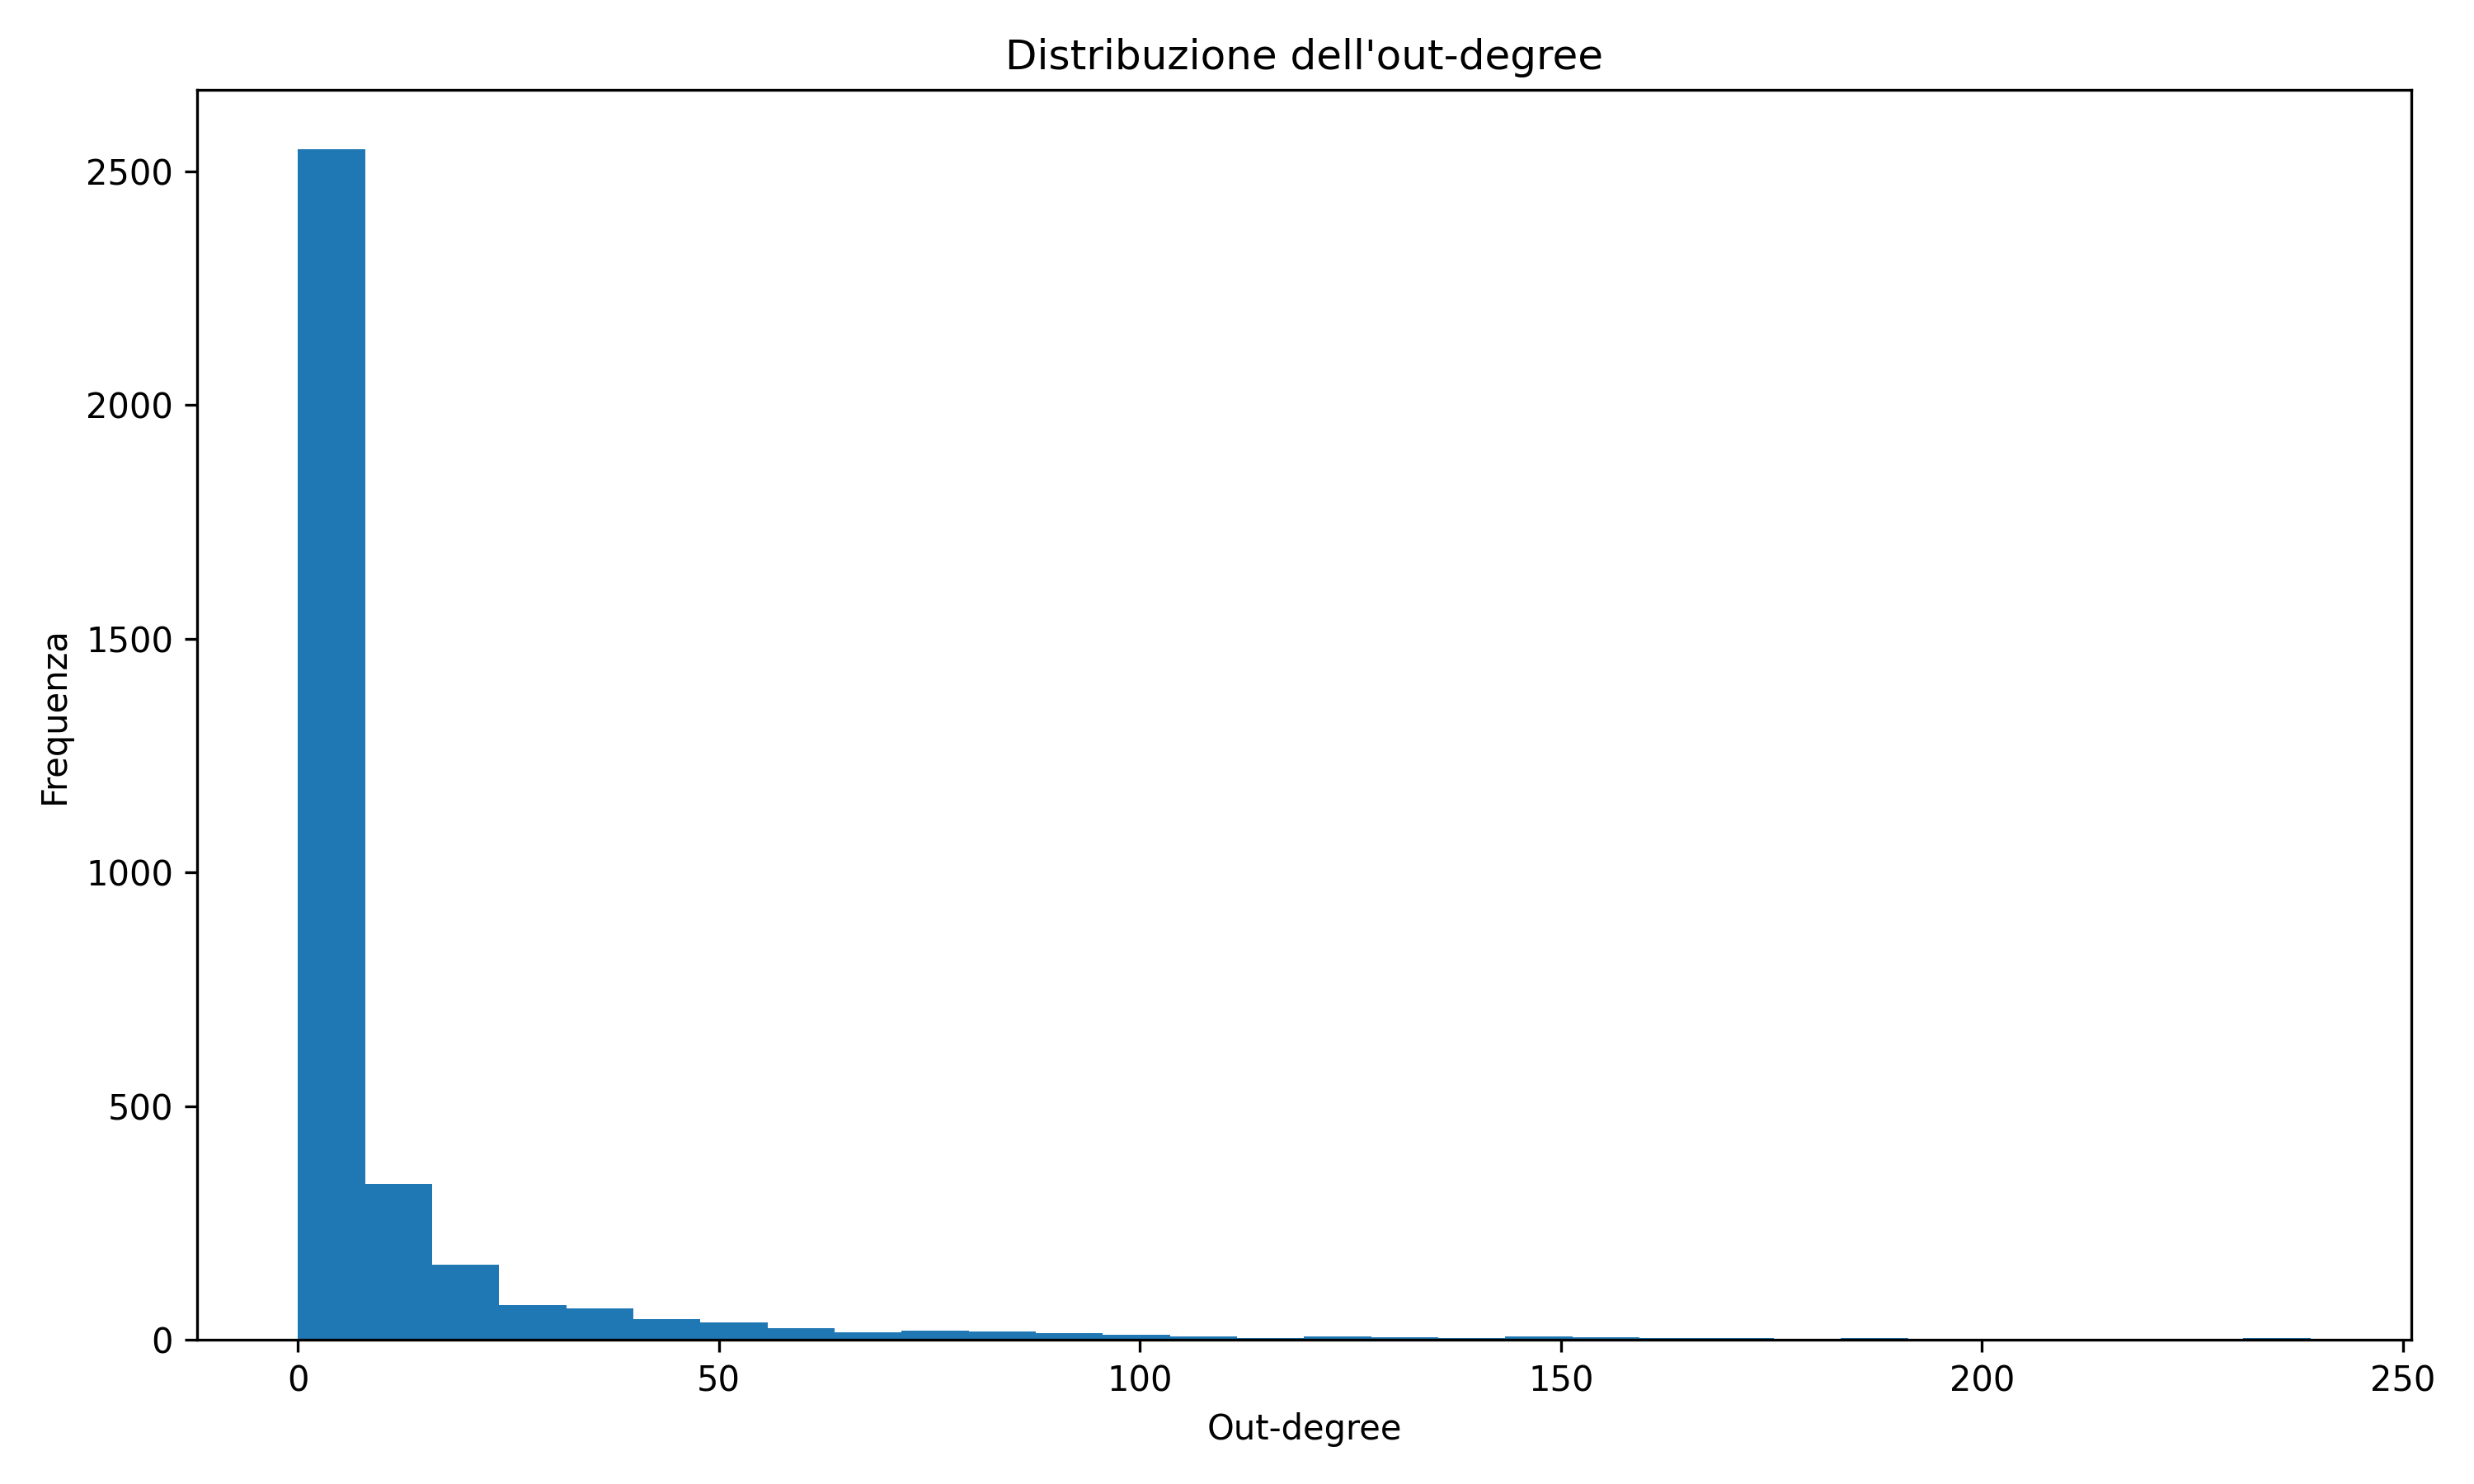
\includegraphics[width=0.9\textwidth]{chapter4/immagini/out_degree_distribution.png}
\caption{Distribuzione dell’out-degree nel grafo diretto.}
\label{fig:out_degree_distribution}
\end{figure}

Le Figure~\ref{fig:in_degree_distribution} e~\ref{fig:out_degree_distribution} evidenziano una concentrazione molto forte dei nodi nelle classi di grado più basse. Questo significa che la gran parte degli aeroporti è collegata direttamente solo a pochi altri scali, mentre esiste una coda lunga composta da aeroporti con numerosi collegamenti.

Per osservare meglio questo andamento, è stata considerata anche una rappresentazione in scala log-log della distribuzione dell’in-degree.

\begin{figure}[H]
\centering
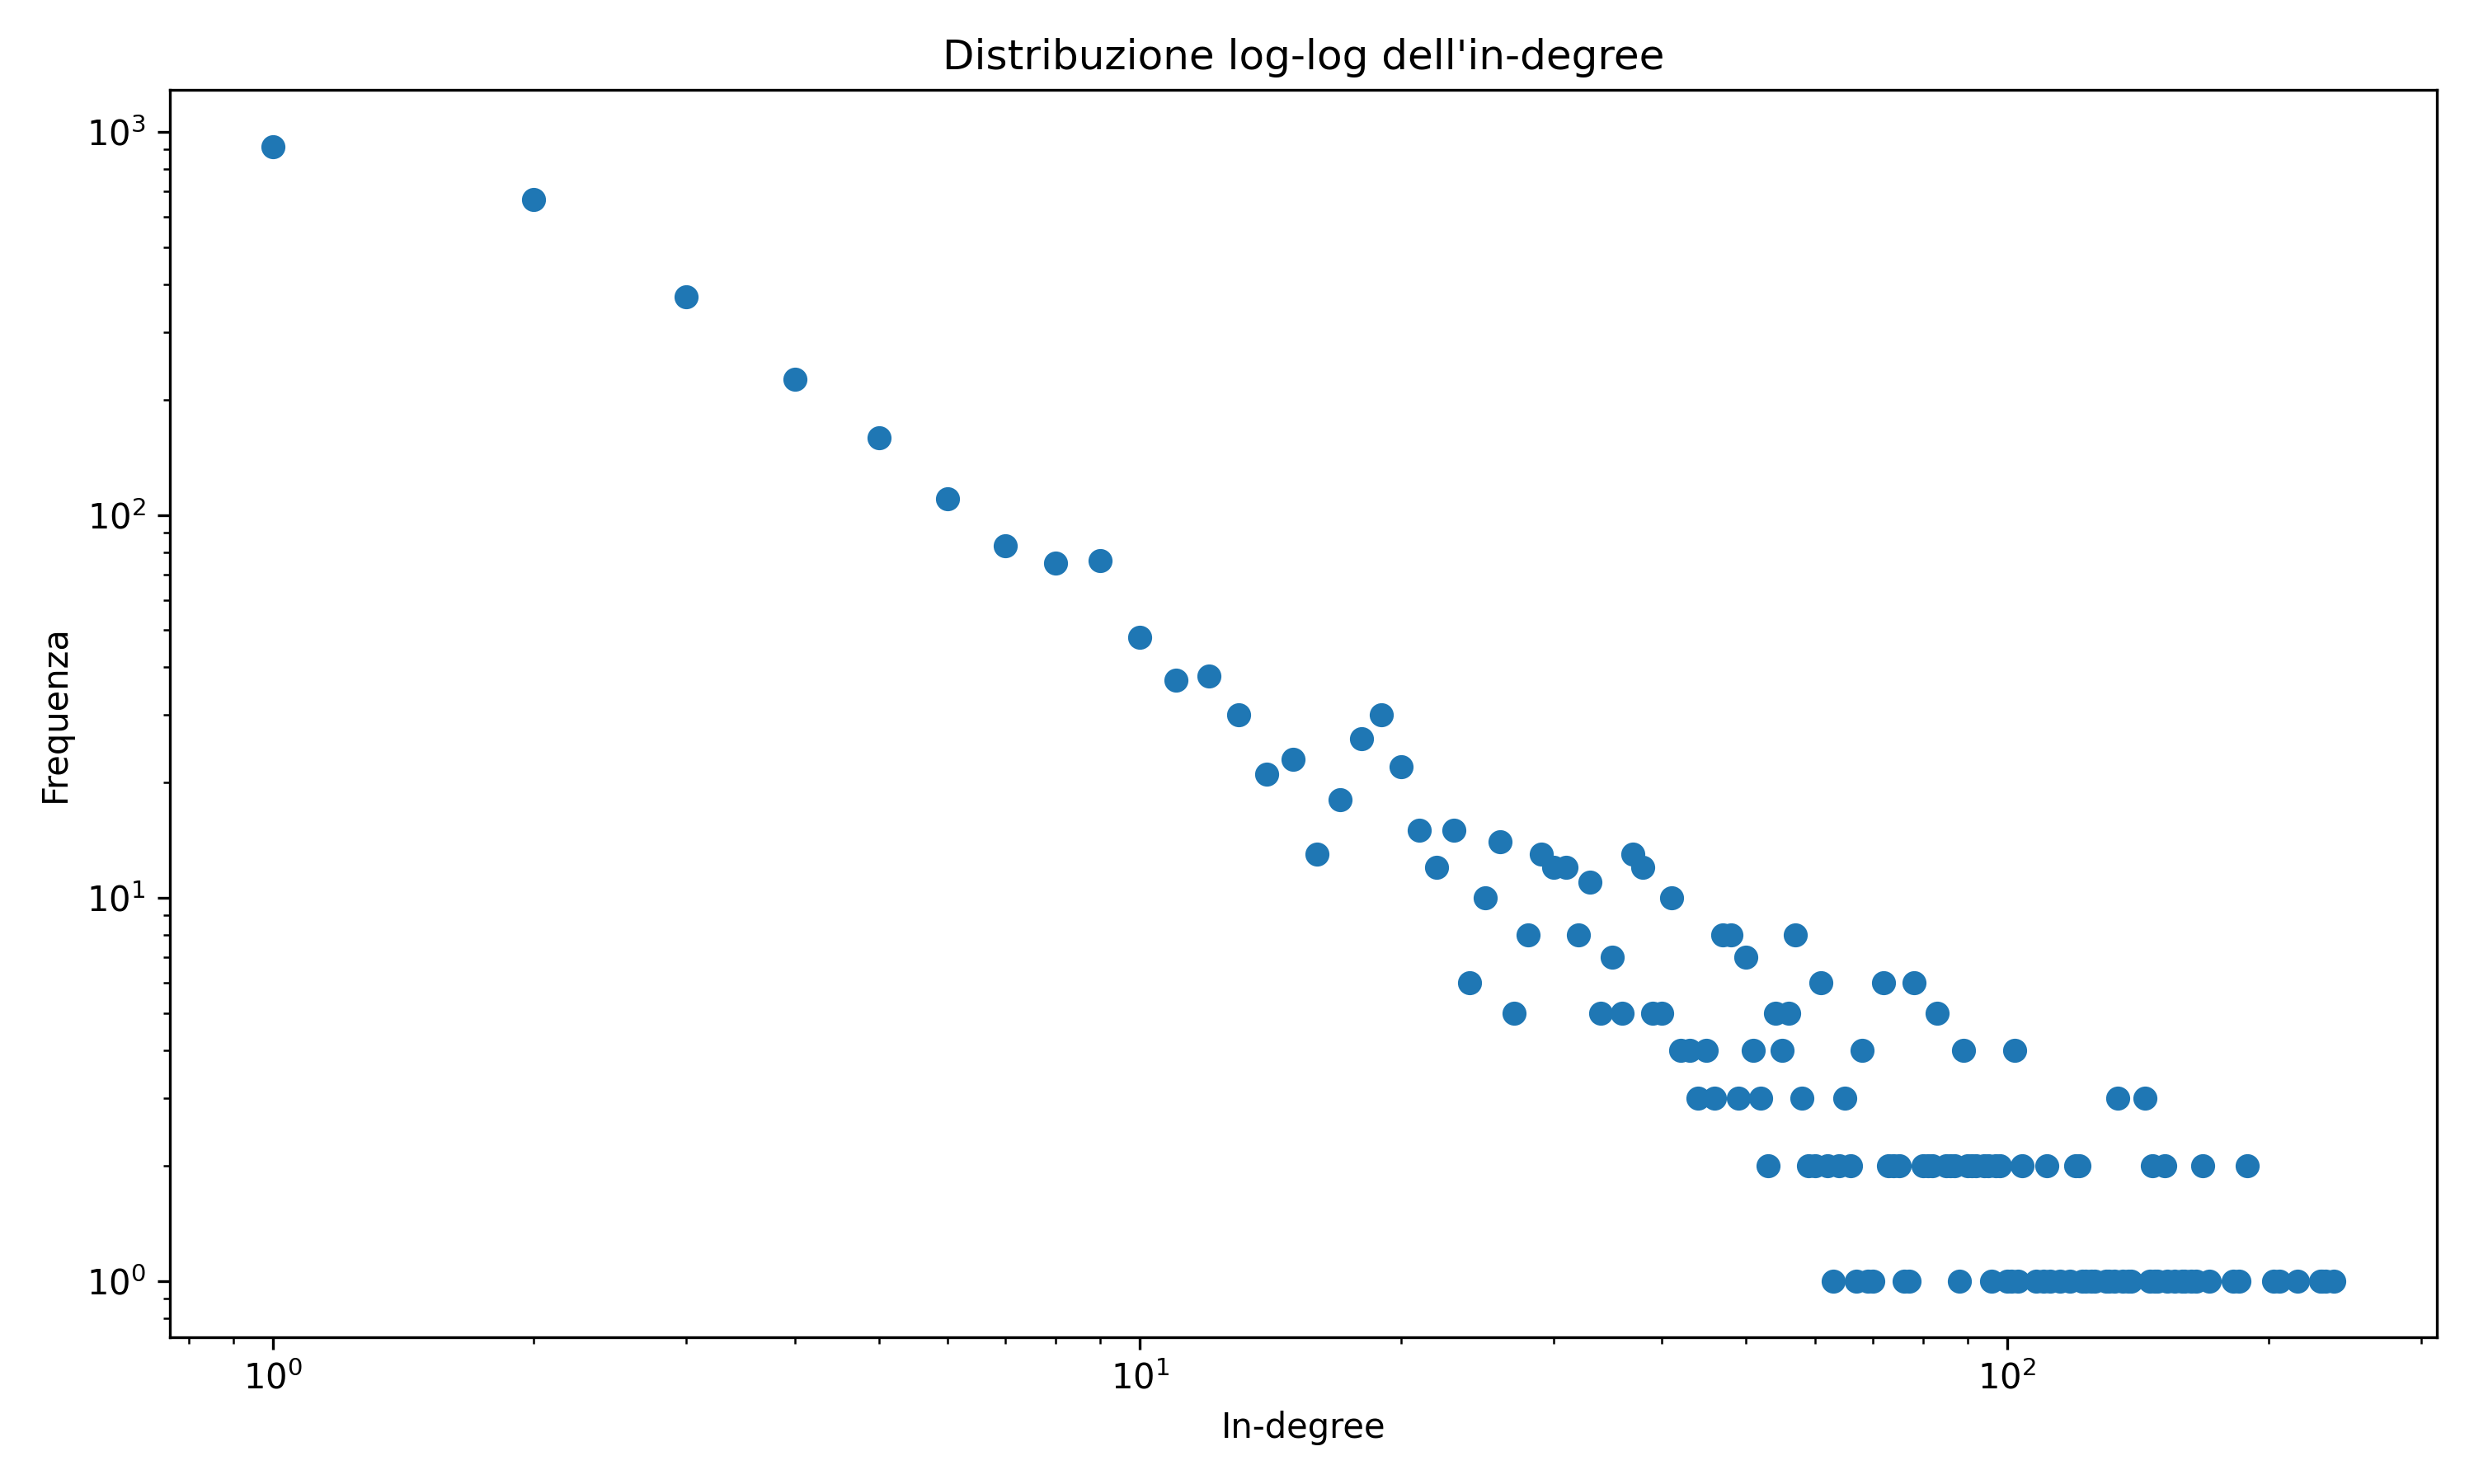
\includegraphics[width=0.9\textwidth]{chapter4/immagini/in_degree_distribution_loglog.png}
\caption{Distribuzione log-log dell’in-degree nel grafo diretto.}
\label{fig:in_degree_distribution_loglog}
\end{figure}

\begin{figure}[H]
\centering
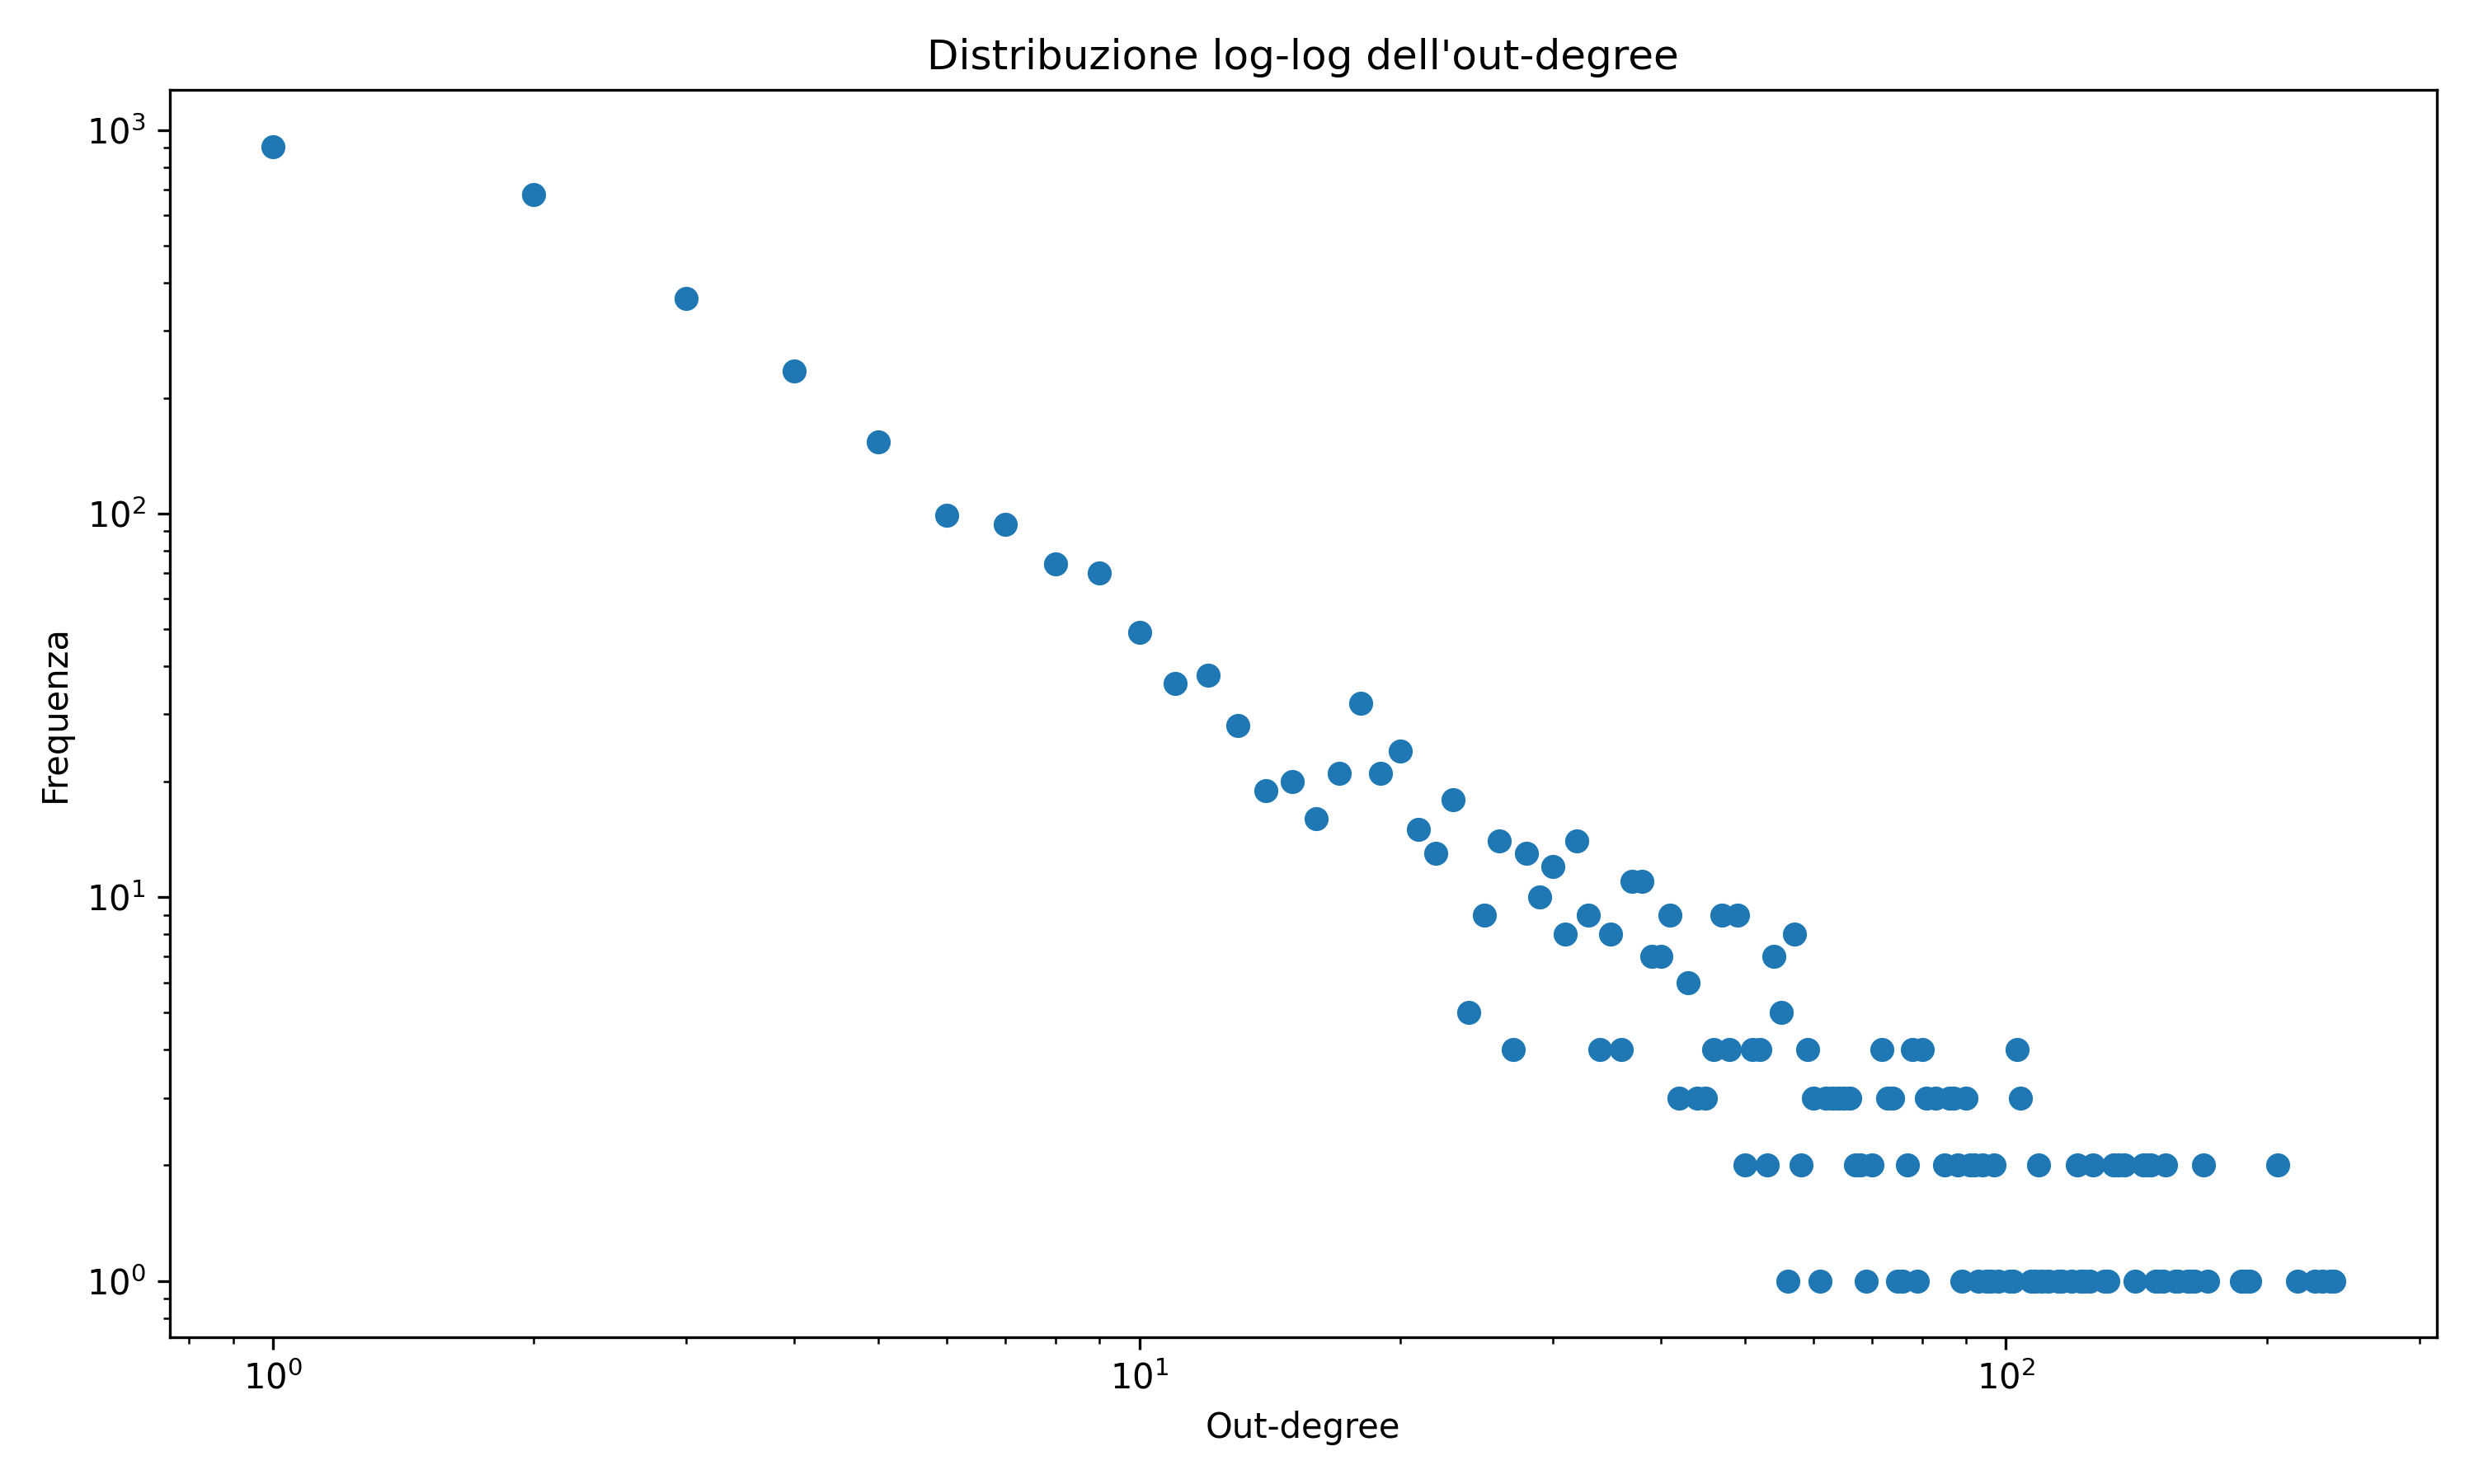
\includegraphics[width=0.9\textwidth]{chapter4/immagini/out_degree_distribution_loglog.png}
\caption{Distribuzione log-log dell’out-degree nel grafo diretto.}
\label{fig:out_degree_distribution_loglog}
\end{figure}

Le Figure~\ref{fig:in_degree_distribution_loglog} e~\ref{fig:out_degree_distribution_loglog} mostrano in modo più chiaro la presenza di una coda lunga in entrambe le distribuzioni, confermando che la rete non presenta una struttura omogenea. Al contrario, essa appare organizzata attorno a pochi aeroporti ad alto grado, tipici di una configurazione di tipo hub-and-spoke.

\section{Aeroporti con maggiore in-degree e out-degree}

Per individuare i nodi più connessi della rete, sono stati ordinati gli aeroporti in base ai rispettivi valori di in-degree e out-degree. I primi dieci aeroporti per ciascuna misura sono riportati nelle Figure~\ref{fig:top_in_degree} e~\ref{fig:top_out_degree}.

\begin{figure}[H]
\centering
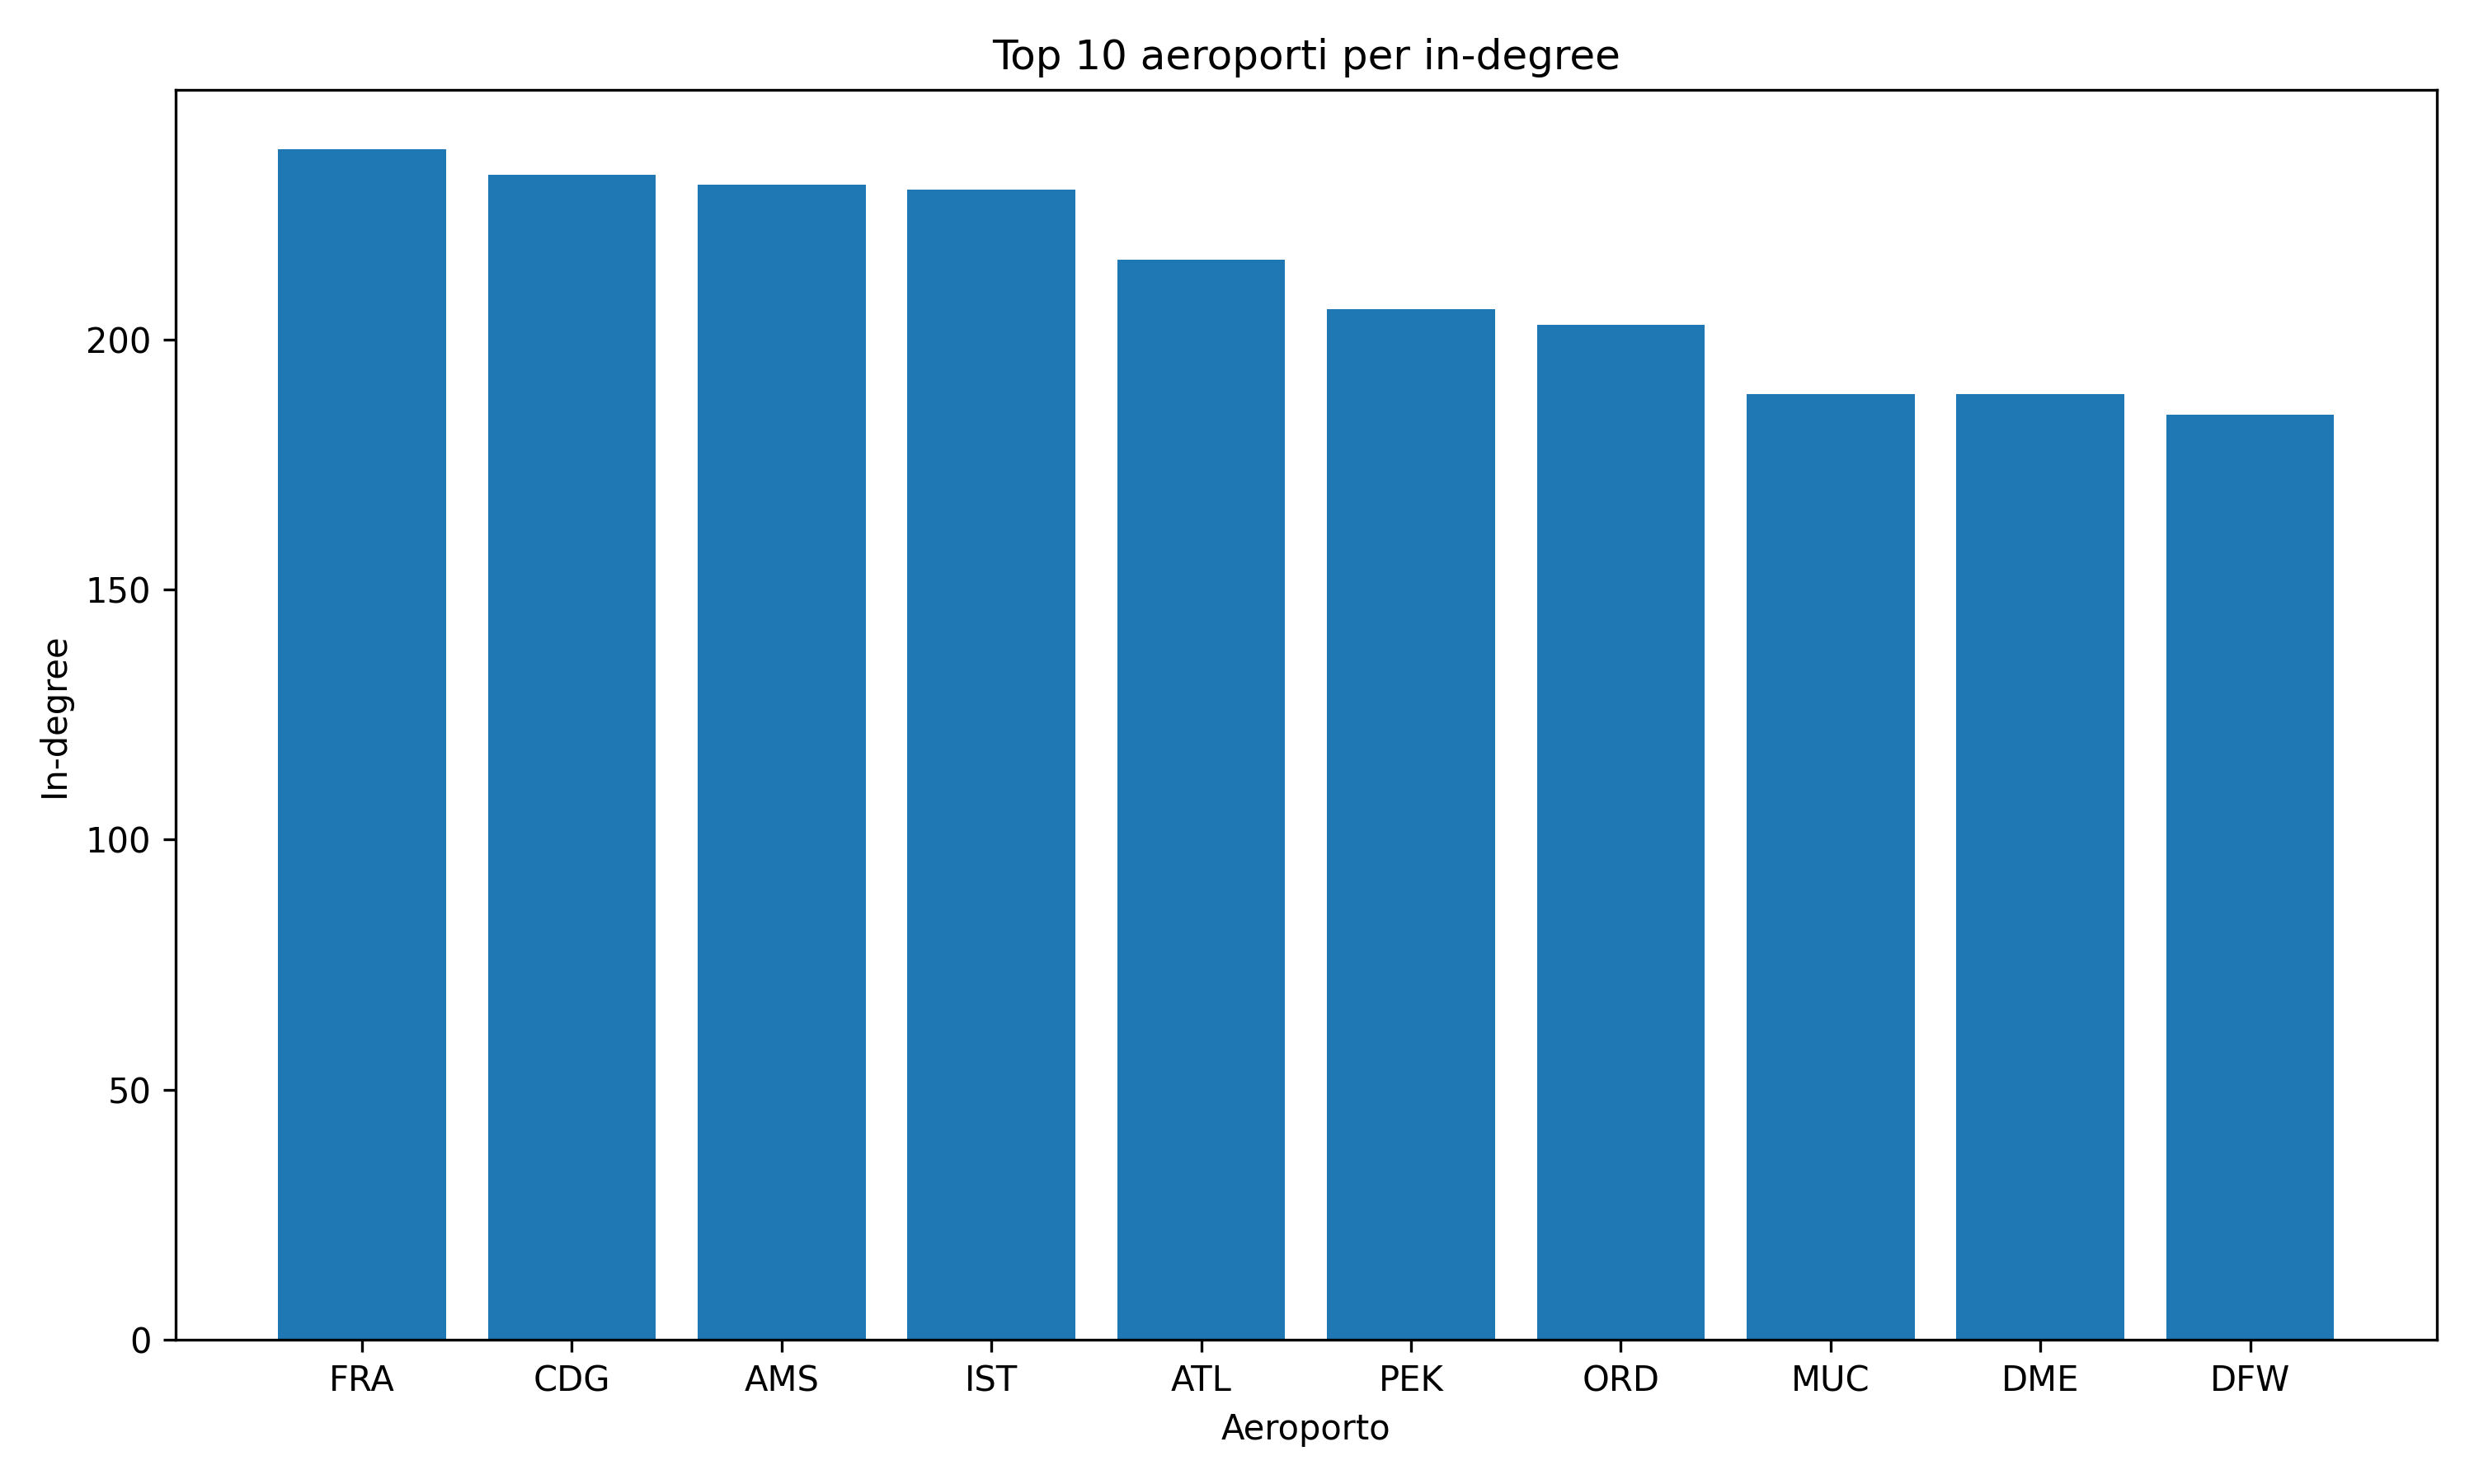
\includegraphics[width=0.9\textwidth]{chapter4/immagini/top10_in_degree.png}
\caption{Top 10 aeroporti per in-degree nel grafo diretto.}
\label{fig:top_in_degree}
\end{figure}

\begin{figure}[H]
\centering
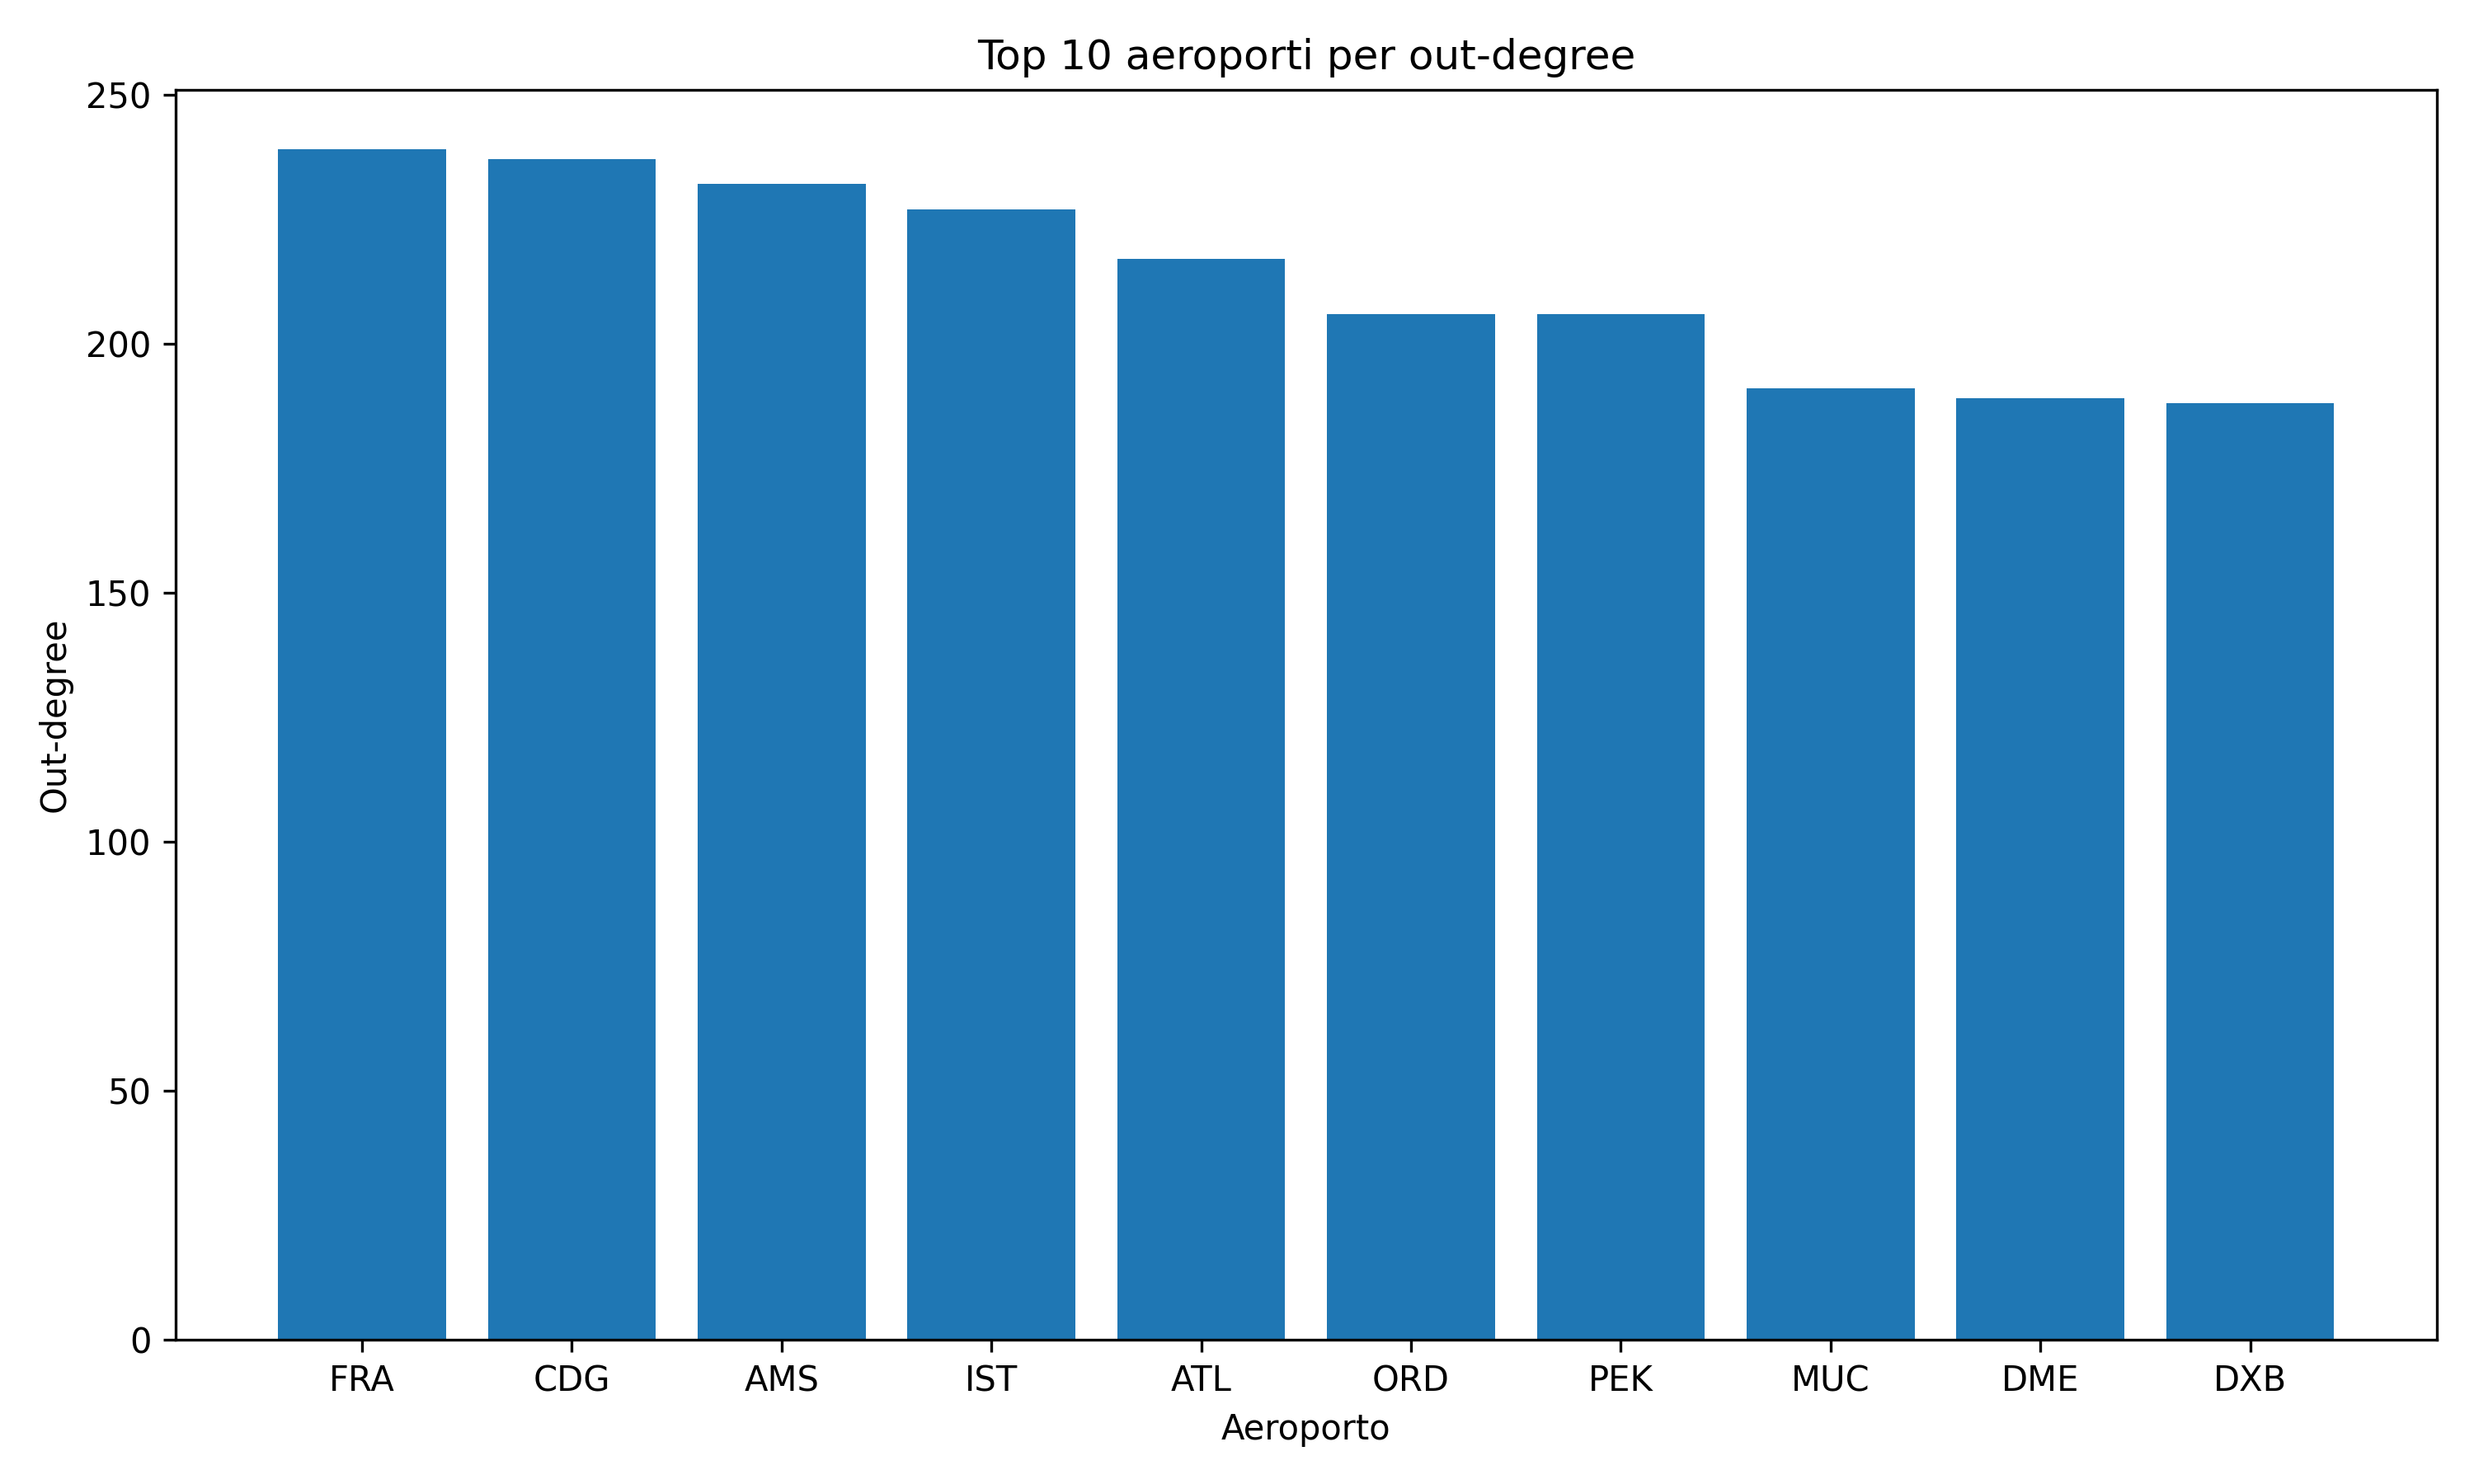
\includegraphics[width=0.9\textwidth]{chapter4/immagini/top10_out_degree.png}
\caption{Top 10 aeroporti per out-degree nel grafo diretto.}
\label{fig:top_out_degree}
\end{figure}

Nel caso dell’in-degree, i primi nodi risultano essere FRA, CDG, AMS, IST e ATL, seguiti da PEK, ORD, MUC, DME e DFW. Per l’out-degree emergono invece FRA, CDG, AMS, IST e ATL, seguiti da ORD, PEK, MUC, DME e DXB.

Questo risultato è particolarmente interessante perché mostra una forte somiglianza tra i due ranking. Molti dei principali aeroporti della rete sono infatti contemporaneamente nodi con elevata capacità di ricezione e di distribuzione delle connessioni. Ciò suggerisce che tali aeroporti svolgano un ruolo di hub bilanciato all’interno del sistema, fungendo sia da punti di arrivo sia da punti di smistamento verso numerose destinazioni.

\section{Statistiche descrittive dei gradi}

Le statistiche descrittive confermano ulteriormente la forte eterogeneità della rete. Per entrambe le distribuzioni, il valore medio del grado è pari a circa 10.98, mentre la mediana è soltanto pari a 3. Questa differenza marcata tra media e mediana indica la presenza di pochi nodi con grado molto elevato, capaci di spostare verso l’alto la media complessiva.

Anche la deviazione standard risulta elevata, pari a circa 24.13 per l’in-degree e 24.21 per l’out-degree. I valori massimi raggiungono 238 per l’in-degree e 239 per l’out-degree, mentre i valori minimi sono pari a 0 in entrambi i casi. Nel complesso, queste grandezze descrivono una rete altamente sbilanciata, in cui coesistono aeroporti periferici con pochissimi collegamenti e nodi centrali dotati di un numero molto elevato di connessioni.

\section{Relazione tra misure topologiche di base}

Per completare l’analisi esplorativa, sono state rappresentate alcune relazioni tra misure topologiche di base, in modo da osservare visivamente eventuali dipendenze tra grado e indicatori di centralità.

\begin{figure}[H]
\centering
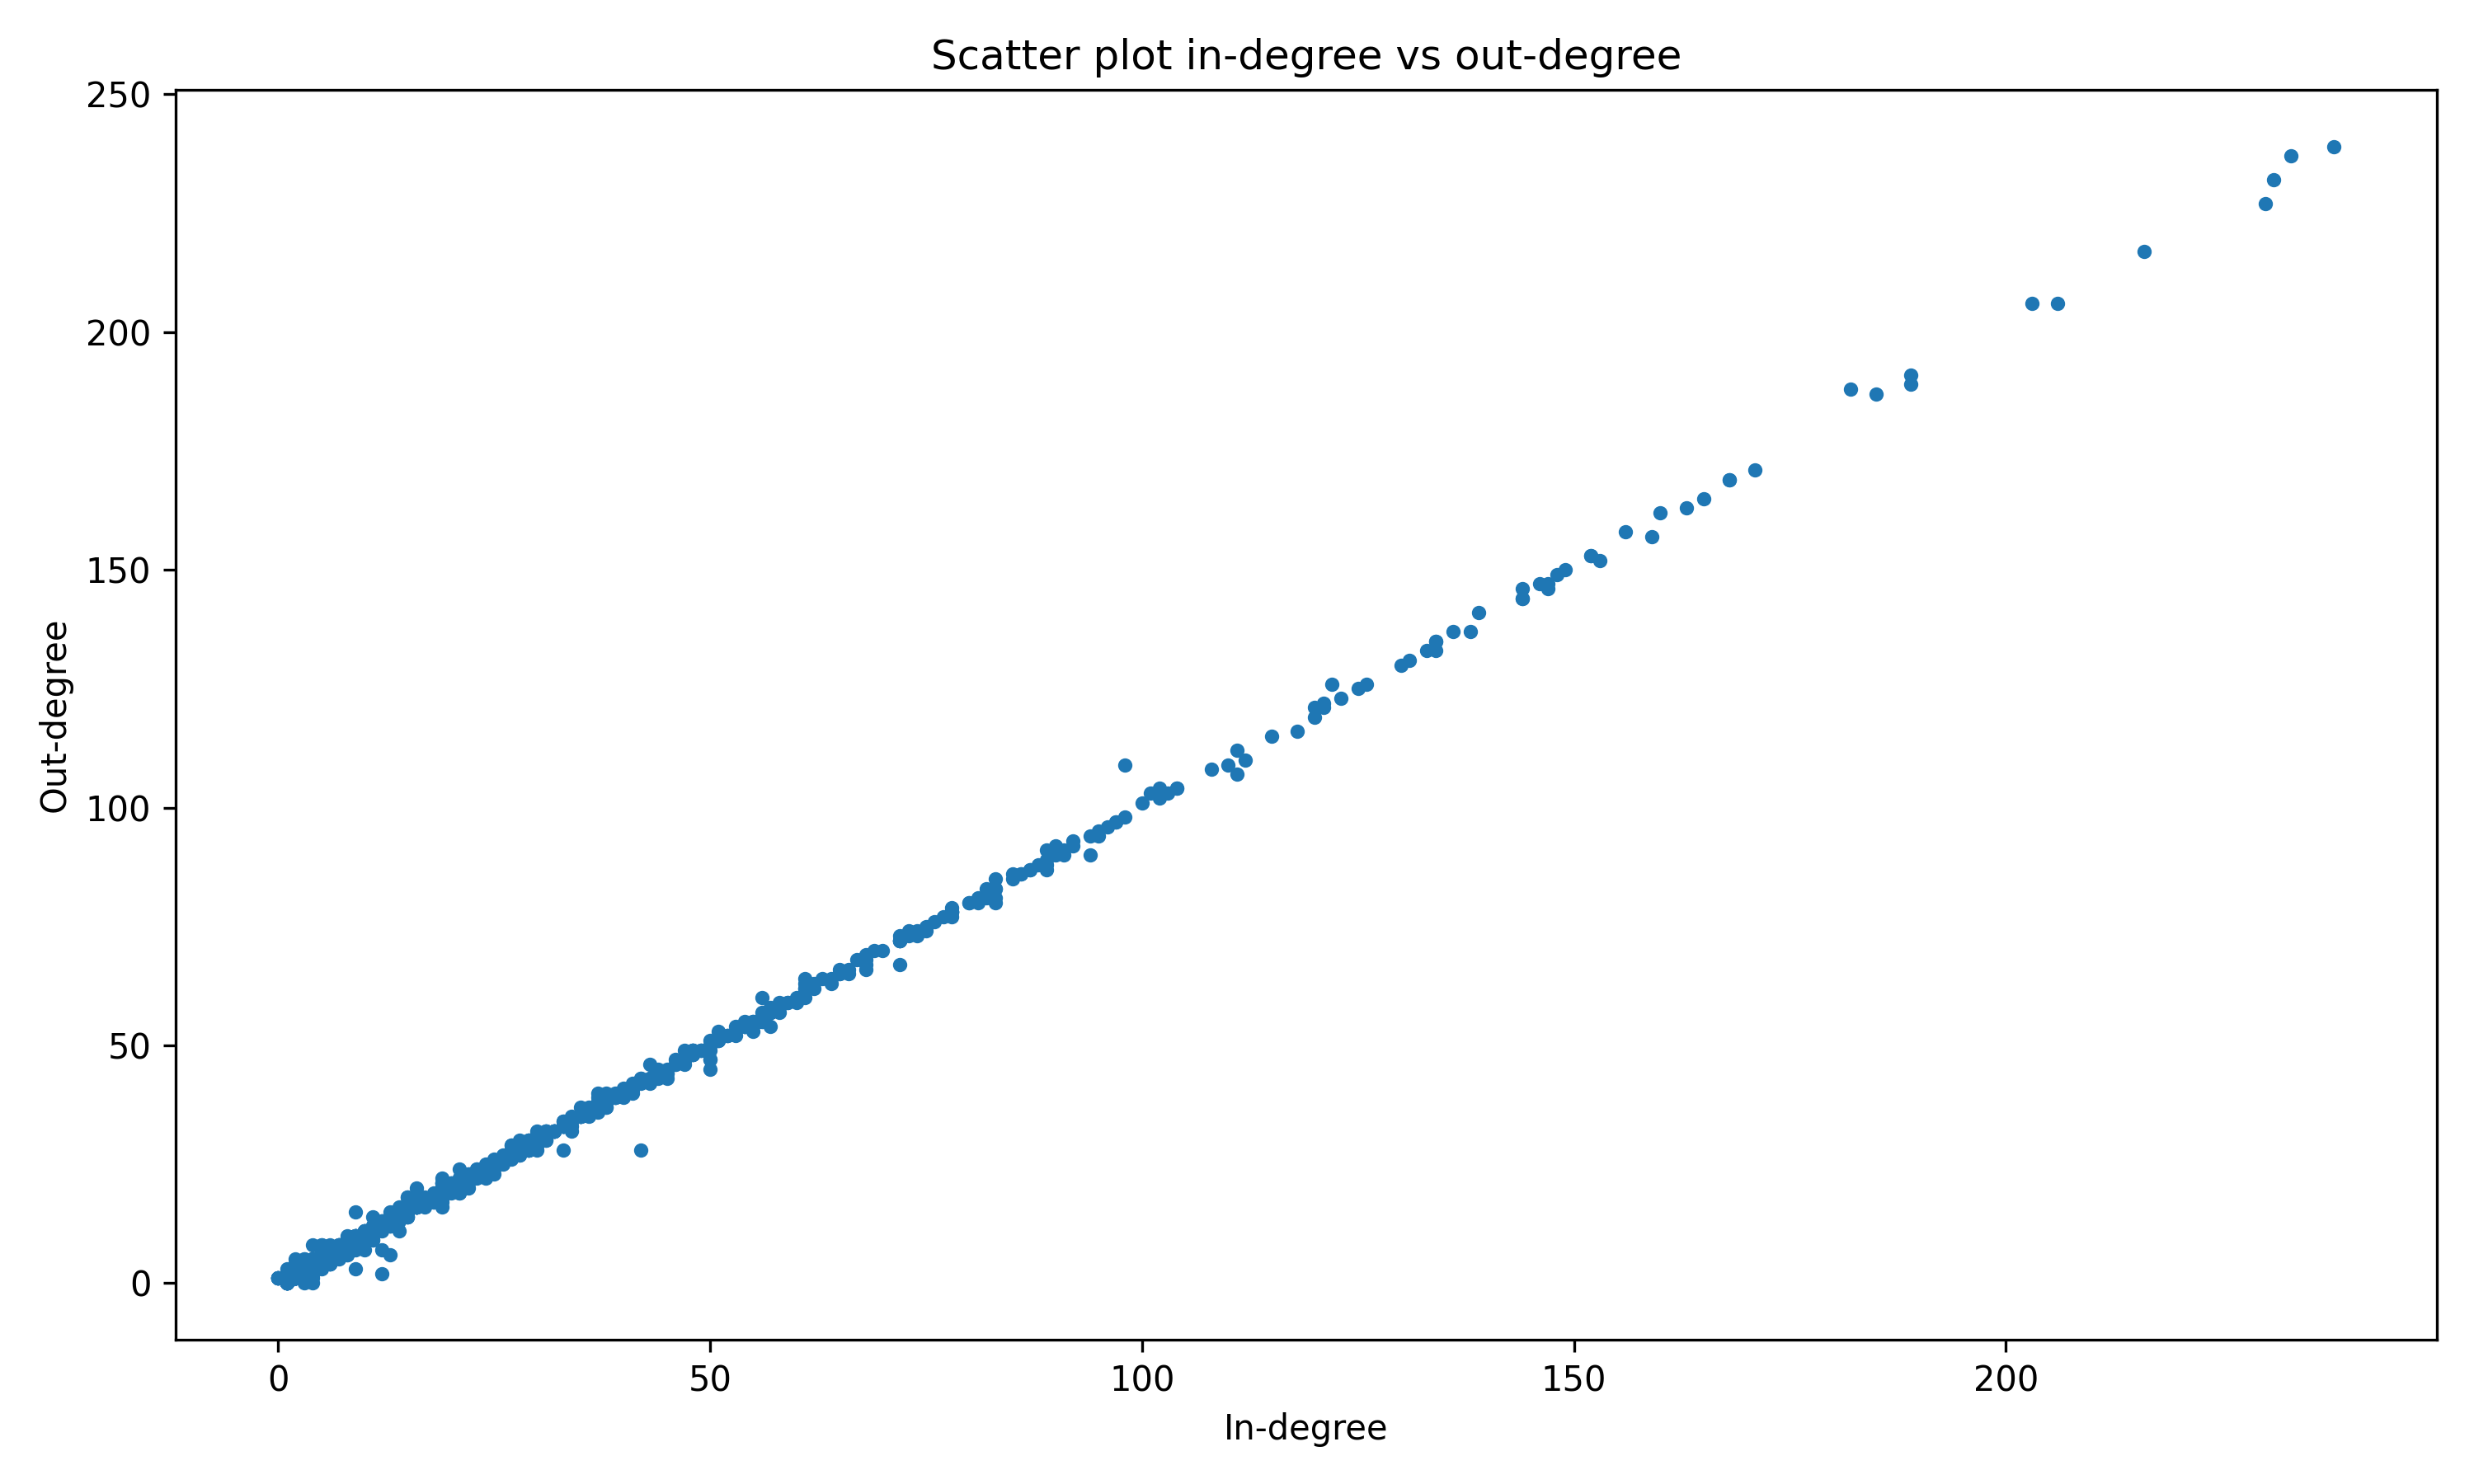
\includegraphics[width=0.9\textwidth]{chapter4/immagini/scatter_in_out_degree.png}
\caption{Scatter plot tra in-degree e out-degree.}
\label{fig:scatter_in_out_degree}
\end{figure}

La Figura~\ref{fig:scatter_in_out_degree} mostra una relazione quasi lineare tra in-degree e out-degree. Questo conferma che, nella rete analizzata, gli aeroporti che ricevono molte connessioni tendono in generale anche a distribuirne molte. Il comportamento osservato è coerente con la natura degli hub aeroportuali, che svolgono simultaneamente funzioni di raccolta e smistamento del traffico.

\begin{figure}[H]
\centering
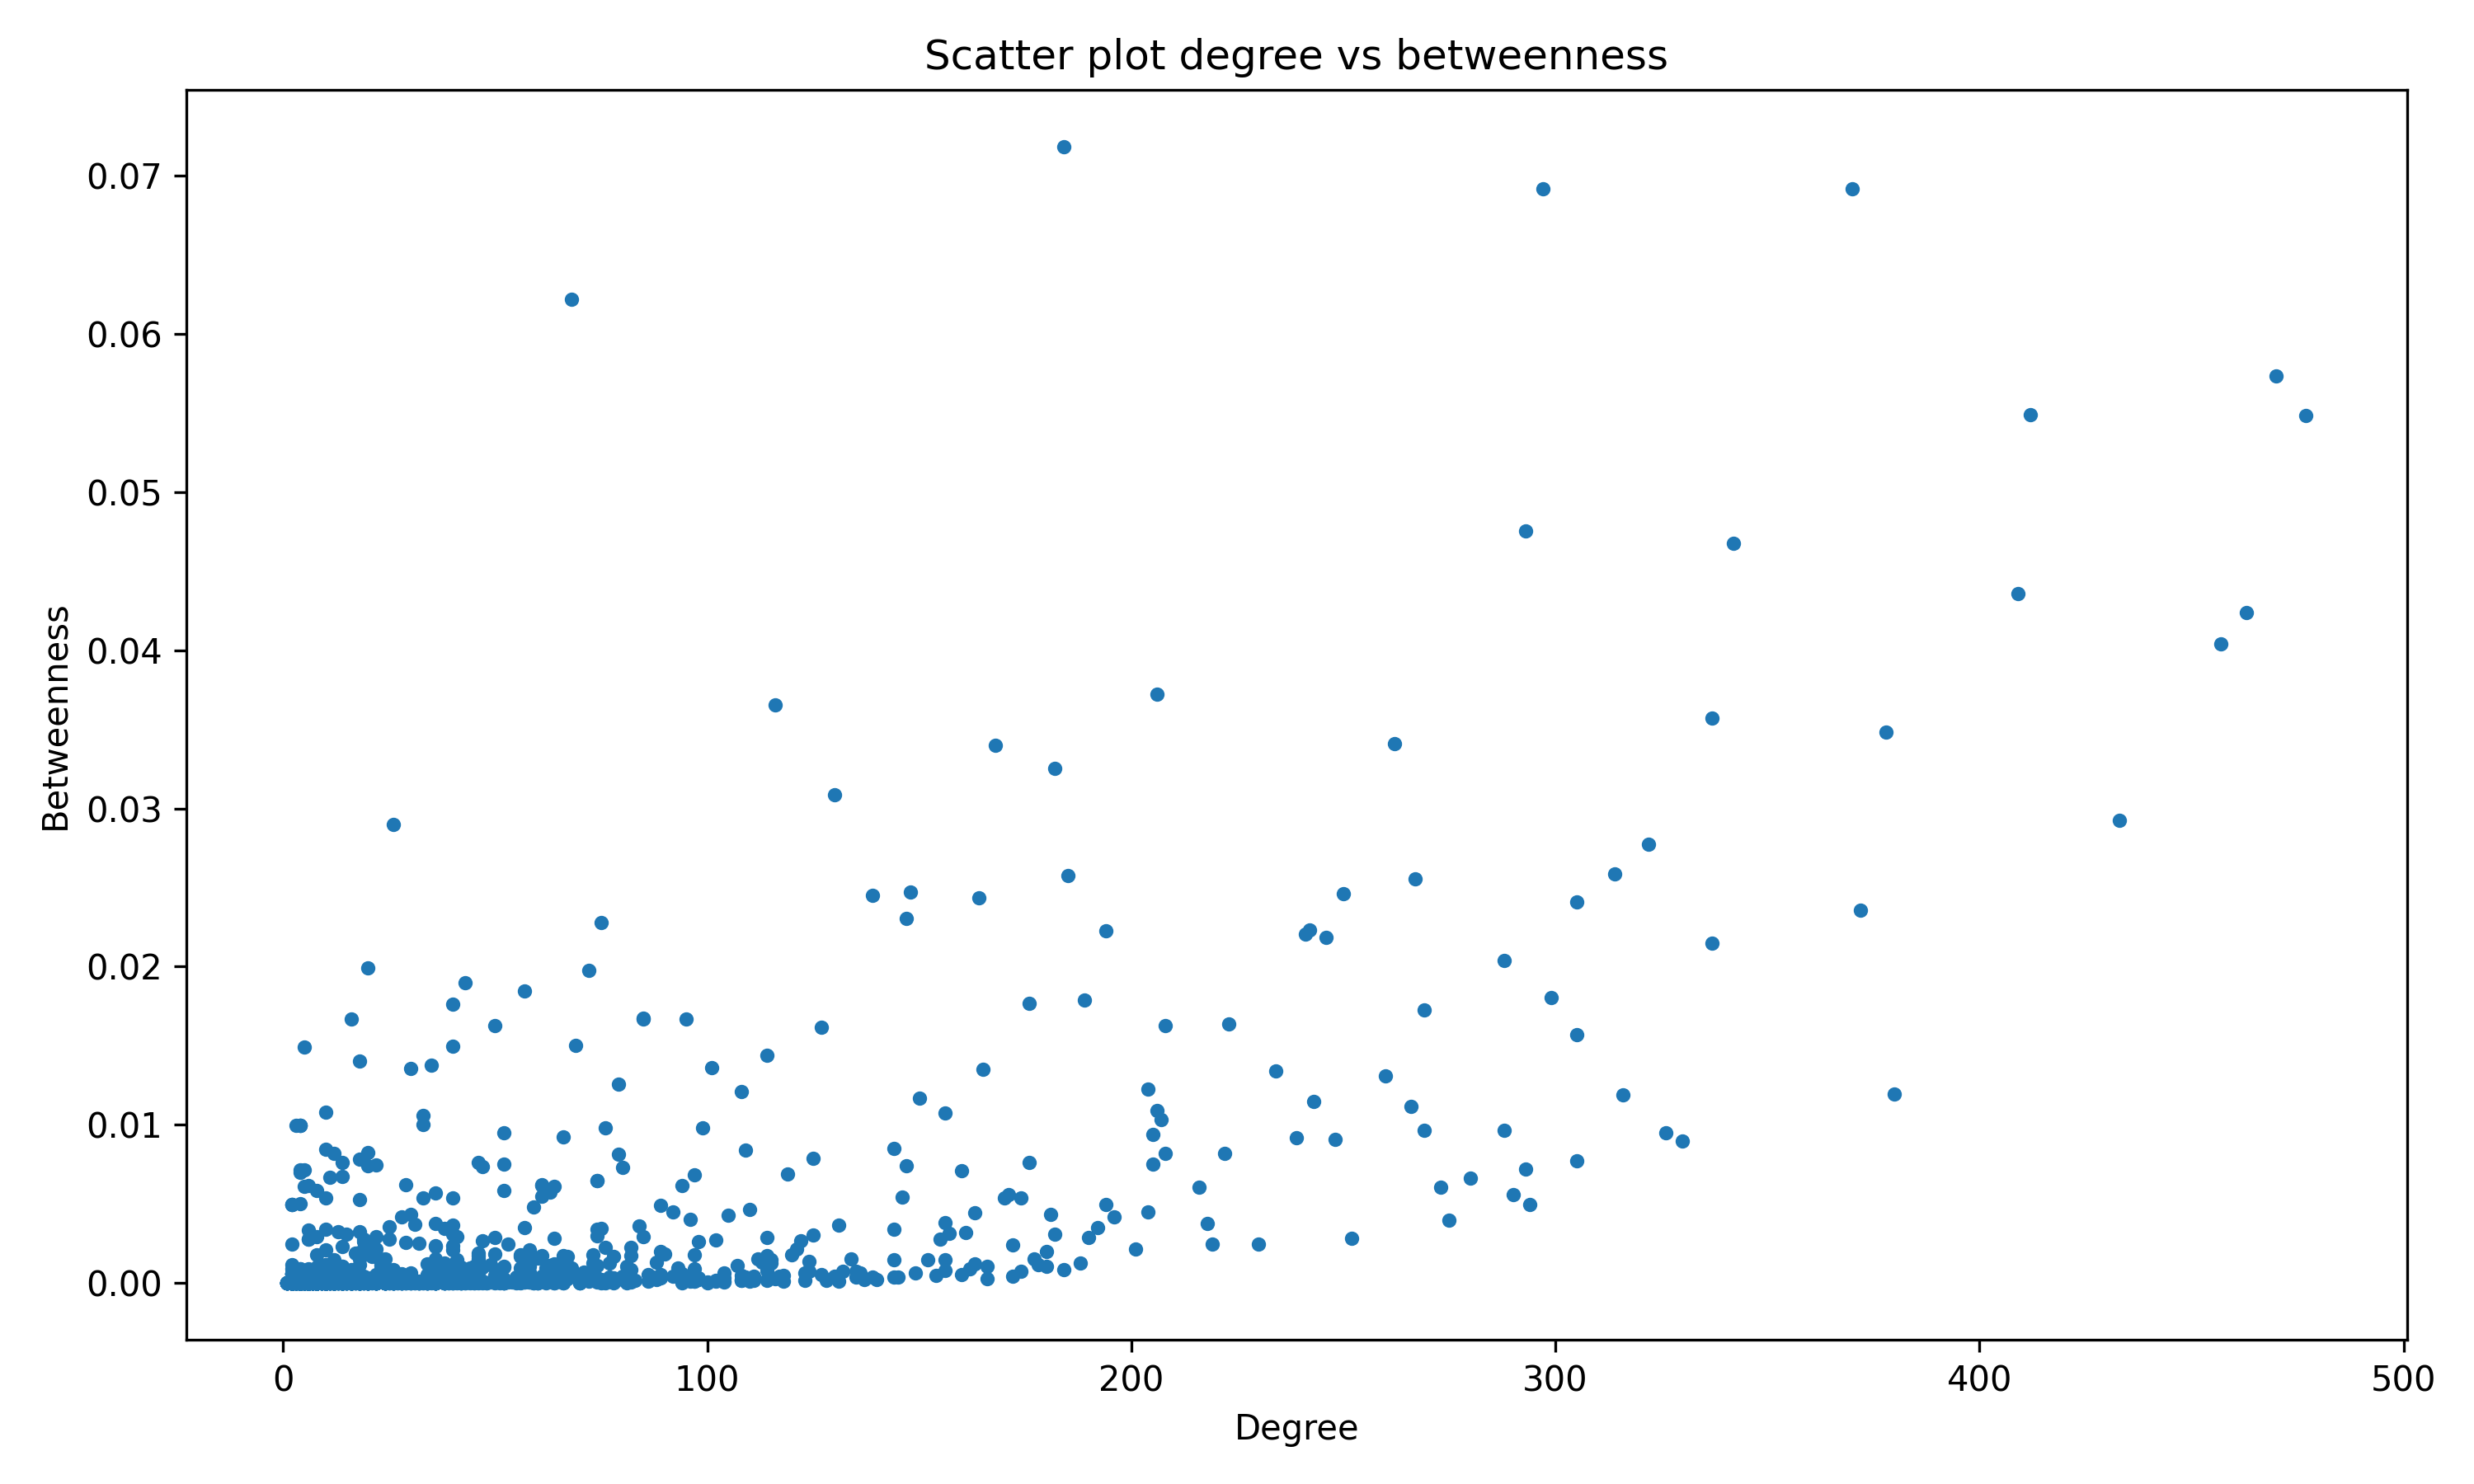
\includegraphics[width=0.9\textwidth]{chapter4/immagini/scatter_degree_betweenness.png}
\caption{Scatter plot tra degree e betweenness centrality.}
\label{fig:scatter_degree_betweenness}
\end{figure}

\begin{figure}[H]
\centering
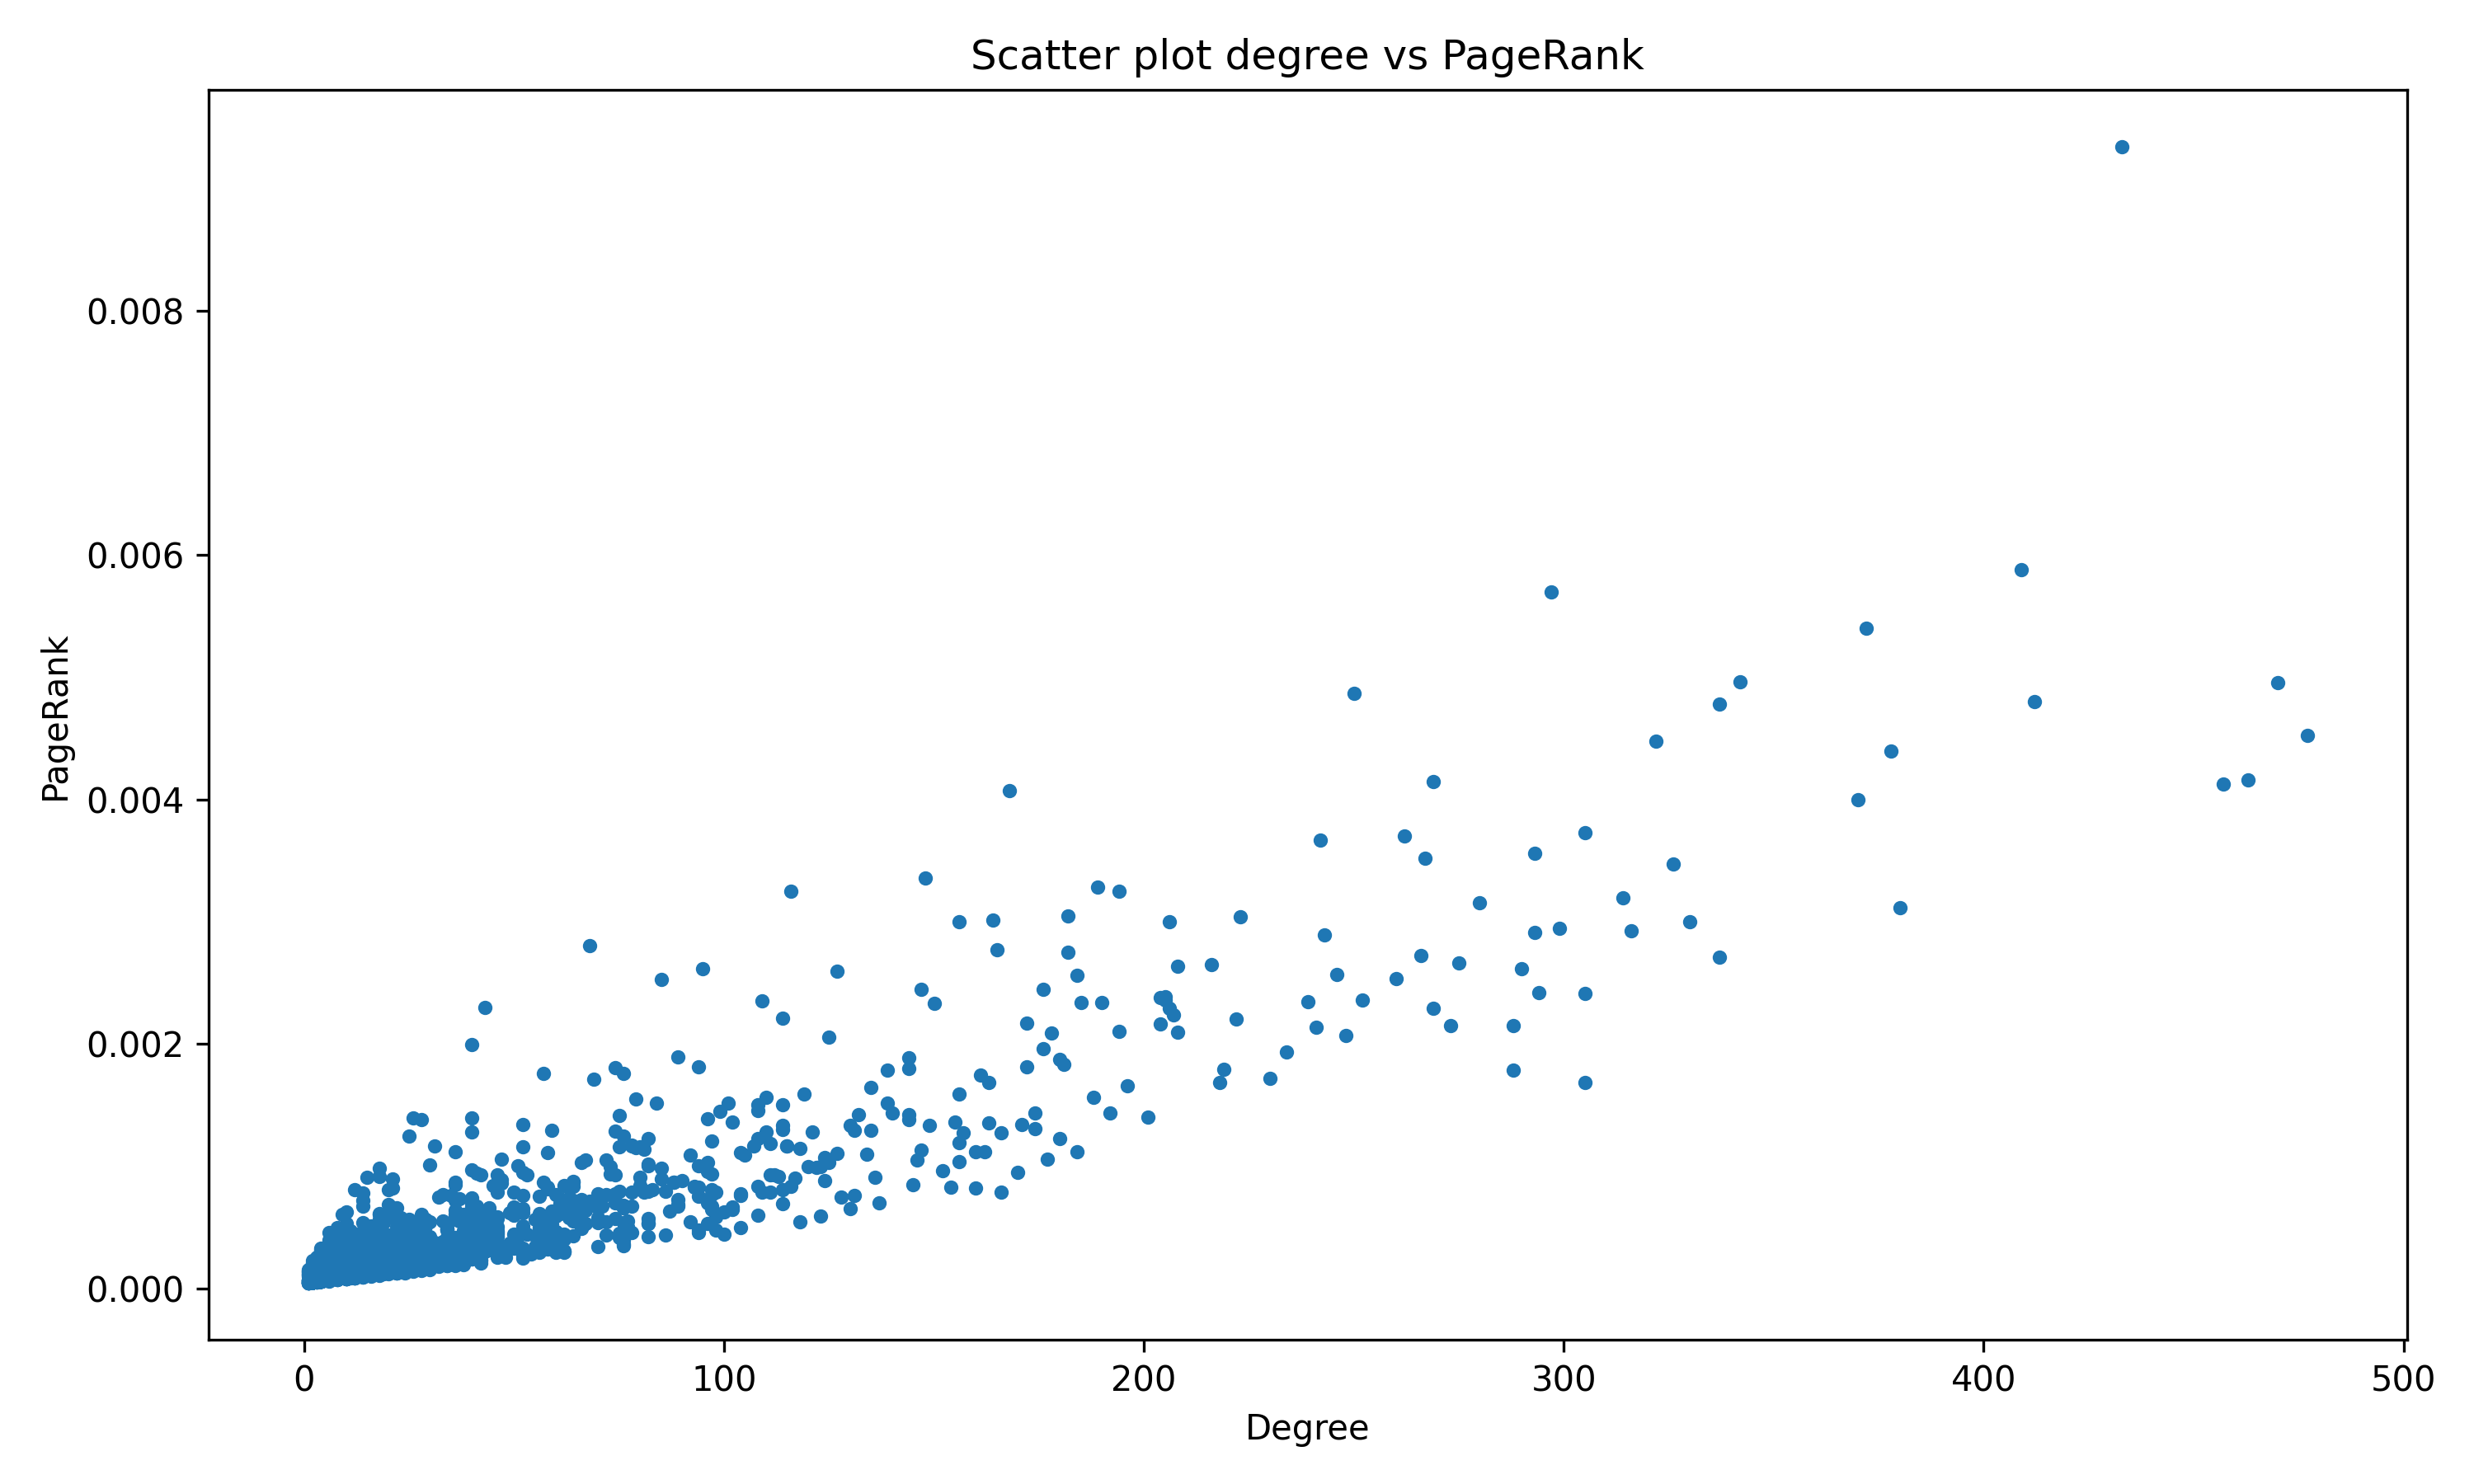
\includegraphics[width=0.9\textwidth]{chapter4/immagini/scatter_degree_pagerank.png}
\caption{Scatter plot tra degree e PageRank.}
\label{fig:scatter_degree_pagerank}
\end{figure}

Le Figure~\ref{fig:scatter_degree_betweenness} e~\ref{fig:scatter_degree_pagerank} mostrano invece che la relazione tra degree e misure di centralità più sofisticate non è puramente lineare. In particolare, la dispersione osservata nel grafico degree--betweenness suggerisce che un nodo molto connesso non è necessariamente anche un forte nodo ponte. Il grafico degree--PageRank evidenzia invece una tendenza crescente più ordinata, indicando che i nodi con grado elevato tendono spesso ad avere anche valori alti di PageRank, pur con alcune differenze legate alla qualità strutturale dei collegamenti.

\section{Componenti connesse}

L’analisi delle componenti connesse fornisce ulteriori informazioni sulla struttura globale della rete. Il grafo diretto presenta:
\begin{itemize}
    \item 8 weakly connected components;
    \item 44 strongly connected components.
\end{itemize}

Le dimensioni delle componenti principali risultano fortemente sbilanciate. In particolare:
\begin{itemize}
    \item la largest weakly connected component contiene 3397 nodi e 37547 archi;
    \item la largest strongly connected component contiene 3354 nodi e 37492 archi.
\end{itemize}

Questi risultati mostrano la presenza di una \textit{giant component} dominante, che comprende quasi tutti i nodi della rete. Le altre componenti hanno invece dimensioni molto ridotte, con la seconda weakly connected component di dimensione 10 e le restanti ancora più piccole.

Dal punto di vista interpretativo, ciò significa che la quasi totalità del sistema aeroportuale considerato appartiene a una struttura fortemente integrata. In altre parole, la rete non appare frammentata in molti sottosistemi indipendenti, ma dominata da un’unica grande componente che raccoglie la maggior parte degli aeroporti e delle connessioni disponibili.

\section{Osservazioni conclusive sull’analisi esplorativa}

L’analisi esplorativa del grafo mette in evidenza alcune proprietà fondamentali della rete delle rotte aeree. In primo luogo, la rete risulta molto ampia ma allo stesso tempo sparsa, come mostrato dal basso valore della densità. In secondo luogo, la distribuzione dei gradi è fortemente asimmetrica e caratterizzata da una lunga coda, segnale tipico della presenza di hub.

Le visualizzazioni globali della rete e delle sue componenti principali rafforzano questa interpretazione, mostrando una struttura fortemente concentrata attorno a un nucleo centrale con numerosi nodi periferici distribuiti ai margini. Inoltre, gli scatter plot tra degree e altre misure topologiche mostrano che il numero di connessioni, pur essendo una caratteristica importante, non esaurisce da solo il ruolo strutturale dei nodi.

I ranking di in-degree e out-degree mostrano che aeroporti come FRA, CDG, AMS, IST e ATL occupano posizioni centrali già a livello puramente topologico. Infine, lo studio delle componenti conferma che la rete è dominata da una componente principale molto grande, segno di un sistema globale fortemente interconnesso.

\begin{table}[H]
\centering
\caption{Sintesi delle principali osservazioni emerse dall’analisi esplorativa.}
\label{tab:exploratory_findings}
\begin{tabular}{ll}
\toprule
\textbf{Aspetto analizzato} & \textbf{Osservazione principale} \\
\midrule
Densità & Rete molto sparsa \\
Distribuzione dei gradi & Presenza di lunga coda \\
Ranking degree & Presenza di hub dominanti \\
Componenti & Giant component dominante \\
Scatter degree--centrality & Relazioni non sempre lineari \\
\bottomrule
\end{tabular}
\end{table}

Queste osservazioni costituiscono la base per le analisi successive. In particolare, dopo aver verificato che il numero di connessioni non è distribuito in modo uniforme e che esistono nodi chiaramente privilegiati, risulta naturale approfondire il ruolo strutturale dei singoli aeroporti attraverso le misure di centralità, che verranno discusse nel capitolo seguente.